%\vspace{3cm}

% \textbf{Àlex Giménez-Romero$^{1}$, Eduardo Moralejo$^{2}$, Manuel A.
%     Matías$^{1}$}

% \vspace{1cm}

% \begin{enumerate}
%     \small
%     \item Instituto de Física Interdisciplinar y Sistemas Complejos, IFISC
%           (CSIC-UIB), Palma de Mallorca 07122, Spain
%     \item Tragsa, Passatge Cala Figuera 6, 07009 Palma de Mallorca, Spain
% \end{enumerate}

% \vspace{1cm}

\textbf{Published as:}

\vspace{0.5cm}

\fullcite{GimenezRomero2023_e}

\newpage
\section{Introduction}

Mathematical and computational modeling in Ecology and, in particular,
Epidemiology have been recently recognized as powerful approaches to guide
empirical work and provide a framework for the synthesis, analysis, and
development of conservation plans and policymaking
\cite{levin1992mathematics,Murray_book,sarkar2006biodiversity,Chew2014}.
Plant epidemics, mainly plant-virus diseases, have often been described by
compartmental models, which deal with the overriding importance of transmission
mechanisms in determining epidemic dynamics
\cite{Jeger1998,Jeger2004,Madden2000}. These models have contributed to
providing answers to some questions related to the ecology of plant diseases
and have led to direct applications in disease control while guiding research
directions \cite{Jeger2019}.

The emergence of vector-borne plant pathogens in new areas causing huge
economic impacts, such as \textit{Xylella fastidiosa} and the
\textit{Candidatus} Liberibacter spp. (Huanglongbing or citrus greening), has
sparked interest in modeling vector-transmitted plant disease epidemics
\cite{chiyaka2012modeling,Jeger2019}. The vector-borne bacterium \textit{X.
    fastidiosa} (Xf) is a multi-host pathogen endemic to the Americas that
causes
economically important diseases, mostly in woody crops \cite{Hopkins2002}. Xf
is a genetically diverse species with three evolutionary well-defined clades
forming the \textit{pauca}, \textit{fastidiosa}, and \textit{multiplex}
subspecies, native from South, Central, and North America, respectively
\cite{Vanhove2019}. Within each subspecies, diverse genetic lineages
with different host ranges are found. Xf is transmitted non-specifically by
xylem-sap-feeding insects belonging to the sharpshooter leafhoppers (Hemiptera:
Cicadellidae, Cicadellinae) and spittlebugs (Hemiptera: Cercopoidae)
\cite{Redak2004}.

Recently, Xf has gained renewed interest due to the massive mortality of
olive trees in Apulia, Italy \cite{Saponari2019}. The first focus of
the olive quick decline syndrome (OQDS) was detected in 2013 around Gallipoli
(Apulia, Italy) \cite{Saponari2013} and since then has spread
throughout the region by the meadow spittlebug, \textit{Philaenus spumarius}.
Although this was the first official detection of Xf in Europe, it has recently
been demonstrated that the pathogen arrived much earlier in Corsica
\cite{Soubeyrand2018} and in the Balearic Islands \cite{Moralejo2020}.
Around 1993, two strains of the subspecies \textit{fastidiosa} (ST1) and
\textit{multiplex} (ST81) were introduced from California to Mallorca (Spain)
with infected almond plants \cite{Moralejo2020}. To date, over 80\% of the
almond trees in Mallorca show leaf scorch symptoms, and the outbreak has
changed the iconic rural landscape of this Mediterranean island
\cite{Olmo2021}.

The meadow spittlebug,	\textit{P. spumarius} (Hemiptera: Aphrophoridae),
has recently been shown to be the main vector of Xf in Europe both in
transmission experiments and in field studies
\cite{Cornara2017,Cornara2018,lopez2022mechanical,Moralejo2019,Saponari2019}.
\textit{P. spumarius} is a polyphagous species from the Palearctic region,
presenting one generation per year (univoltine) and overwintering as eggs.
Foam-forming nymphs emerge at the end of winter, feeding on herbaceous plants.
The time required for their development to the adult stage depends mainly on
temperature and humidity
\cite{bodino2019phenology,Chmiel1979,cornara2018philaenus}. In Mediterranean
climates,  \textit{P. spumarius} adults generally move from the herbaceous
cover to the crop canopy as evapotranspiration increases in late spring
(May–June). In mid-summer, the populations of \textit{P. spumarius} tend to
decrease in the crop canopy, while the insects are captured more frequently in
trees and shrubs interspersed in crops. Summer dispersal of spittlebugs to wild
hosts as refugee seems a common general pattern in Mediterranean crops in Italy
\cite{bodino2019phenology,cornara2021natural} and Spain
\cite{morente2018distribution}. Because the bacterium has not been detected
in spring on insects feeding on the herbaceous cover or in weeds in Europe
\cite{bodino2019phenology,cornara2018philaenus,Olmo2021}, it is assumed that
all spittlebug adults acquire the bacteria from the main crop (olive, almond,
vine, etc.). Once infected, Xf colonizes the insect foregut in a persistent and
non-circulatory manner without transovarial (parent to offspring) or
transstadial (inter-stage) transmission
\cite{Almeida2003,freitag1951host,purcell1979evidence} and without
a period latency after vector acquisition \cite{Almeida2015,freitag1951host}.

Several epidemic models have already been developed for Xf diseases, but
they lack a realistic description of some relevant processes \cite{Jeger2019}.
Some of these models assume a simple general form for infected host dynamics
\cite{White2017,Abboud2019,Daugherty2019} or use a simplified S-I compartmental
scheme for hosts, disregarding important features
such as the latent period or the host mortality rate \cite{Soubeyrand2018}.
Models that do take these features into account, however, do not explicitly
model the population of vectors responsible for disease transmission
\cite{White2020}. Other more recent models have taken a step further in
explicitly modeling the vector population \cite{BRUNETTI2020,
    GimenezRomero2022_CommsBio}, but the characterization of its dynamics is
still
relatively simple, as it overlooks the known seasonal patterns of vector
abundance. Several recent studies have provided new insights into the ecology
and temporal dynamics of the transmission of Xf by \textit{P. spumarius} in
olive plants \cite{Bodino2021,bodino2019phenology}. However, these
experimental data of the pathosystem have not been yet integrated at the
population level. Thus, there is a need to continue advancing in the modeling
of Xf diseases by developing more realistic models that can elucidate the
fundamental processes involved in vector-host-pathogen interactions and help to
design effective control strategies.

In this work, we develop a deterministic continuous-time compartmental
model to describe the general epidemiological dynamics of diseases produced by
Xf in Europe. We explicitly account for key biological aspects of the disease,
including the seasonal dynamics of its main vector, \textit{P. spumarius}. Our
model is able to describe field data from the two major European outbreaks: the
olive quick disease syndrome (OQDS) in Apulia, Italy, caused by the subspecies
\textit{pauca}, and the almond leaf scorch disease (ALSD) in Mallorca, Spain,
caused by subspecies \textit{multiplex} and \textit{fastidiosa}. We aimed to
find the most influential parameters in the model with respect to incidence and
mortality in both diseases by performing a global sensibility analysis. With
this information, the next goal was to explore control strategies acting
especially on the vector population.

\section{Materials and Methods}

\subsection{Epidemic model: the SEIR-V model}

We developed a deterministic continuous-time compartmental model that
incorporates the specific biological features of Xf diseases in Europe,
including the dynamics of the main relevant vector, \textit{P. spumarius}
\cite{Cavalieri2019}. To build the model, we took the following
considerations: (i) we assume there is no winter recovery of infected hosts and
thus they die sometime after infection; (ii) hosts show an asymptomatic period
in which they are non-infectious in practice (exposed compartment) because the
bacteria are not yet systemically extended
\cite{teviotdale2003almond,Stevenson238}, while vectors are infectious
immediately after acquiring the bacterium \cite{Fierro2019}; (iii) vectors
have an annual life cycle without mother-to-offspring disease transmission
\cite{freitag1951host,purcell1979evidence}, so we consider the annual
emergence of susceptible newborn vectors and a constant death rate for both
susceptible and infected vectors; (iv) infected vectors carry the bacterium
during their entire lifespan without affecting their fitness; and finally, (v)
we do not consider host recruitment or natural death given that the typical
development time of Xf-epidemics is faster than the typical host's life cycle.

Altogether, our deterministic continuous-time compartmental model consists
of six compartments, four describing the host population (susceptible, $S_H$,
exposed, $E_H$, infectious, $I_H$, and removed, $R_H$), and two describing the
vector population (susceptible, $S_V$, and infected, $I_V$). The model is
defined according to the following processes,
\begin{equation}\label{eq:scheme_infection_phyto}
    \begin{aligned}
         & S_H+I_V \stackrel{\beta}{\rightarrow} E_H + I_V, \quad
        E_H \stackrel{\kappa}{\rightarrow} I_H, \quad
        I_H  \stackrel{\gamma}{\rightarrow} R_H                      \\
         & S_V+I_H \stackrel{\alpha}{\rightarrow} I_V+I_H, \quad S_V
        \stackrel{\mu}{\rightarrow} \varnothing, \quad I_V
        \stackrel{\mu}{\rightarrow}
        \varnothing
        \ ,
    \end{aligned}
\end{equation}
which are illustrated in \cref{fig:model_diagram_phyto}, being the birth of new
susceptible vectors described as a source term.

\begin{figure}[H]
    \centering
    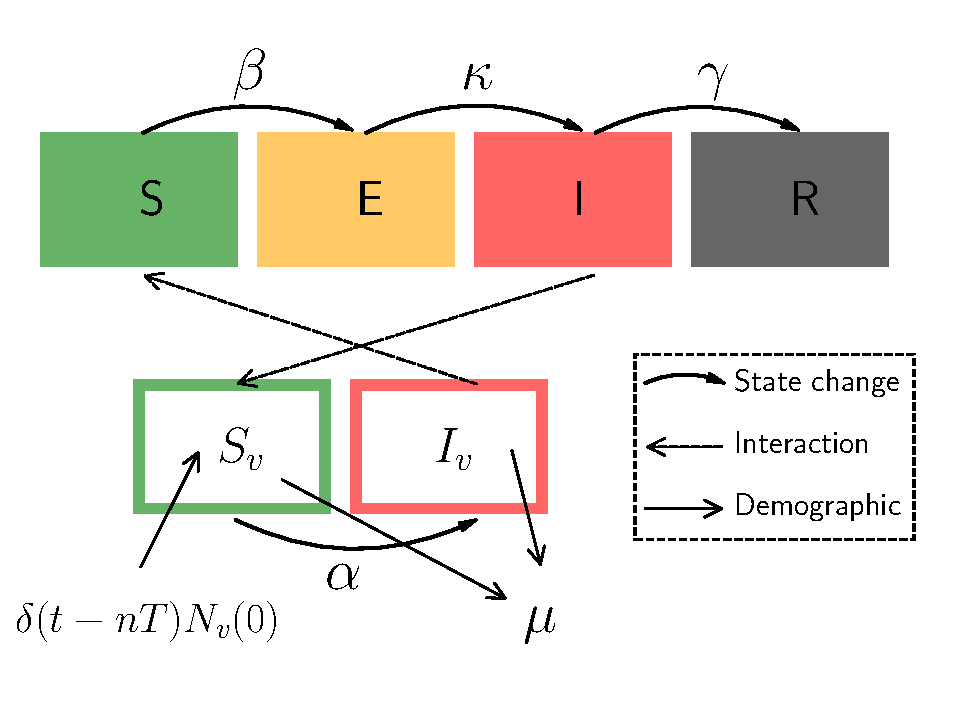
\includegraphics[width=0.95\textwidth]{Figures/SEIR_v_scheme.pdf}
    \caption[Schematic representation of the model]{Schematic representation of
        the model \cref{eq:SEIR_v}. Boxes
        are the compartments in which the population is divided; solid curved
        arrows represent changes in state, i.e., transitions between
        compartments; dashed arrows depict the crossed interaction between
        hosts and vectors; and solid straight arrows represent demographic
        changes in the vector population.}
    \label{fig:model_diagram_phyto}
\end{figure}

The host-vector compartmental model is written as,
\begin{equation}\label{eq:SEIR_v}
    \begin{aligned}
        \dot{S}_H & =-\beta S_H I_v / N_H                                   \\
        \dot{E}_H & =\beta S_H I_v / N_H - \kappa E_H                       \\
        \dot{I}_H & =\kappa E_H - \gamma I_H                                \\
        \dot{R}_H & =\gamma I_H                                             \\
        \dot{S}_v & = N_v(0)\sum_{n=1}^{\infty}\delta(t-nT) -\alpha S_v I_H
        / N_H - \mu S_v                                                     \\
        \dot{I}_v & =\alpha S_v I_H / N_H - \mu I_v \ .
    \end{aligned}
\end{equation}

The model describes the exposure of susceptible hosts, $S_H$, at a rate
$\beta$ through their interaction with infected vectors, $I_v$, while
susceptible vectors, $S_v$, get infected immediately at a rate $\alpha$ through
their interaction with infectious hosts $I_H$. Exposed hosts get infectious at
rate $\kappa$, having a mean latent period $\tau_E=1/\kappa$, while infectious
hosts die at rate $\gamma$, having a mean infectious period of
$\tau_I=1/\gamma$. Infected vectors stay infected and infectious for the rest
of their lifetime.

Regarding the seasonal dynamics of vectors, we assume that
new adults emerge synchronously each year in fields being all susceptible. This
is represented by the term $N_v(0)\sum_{n=1}^{\infty}\delta(t-nT)$ in
\cref{eq:SEIR_v}, where $T=\SI{1}{yr}$ is the period and $\delta(t-nT)$ is the
Dirac delta function, and basically implements a yearly pulse of new vectors at
a certain moment in the year. Vectors are removed (die, move to herbaceous
vegetation and other non-host trees, exit the field, etc.) at a given rate
$\mu$, which we consider identical for susceptible and infected vectors. For
simplicity, we consider that the quantity of annual newborn adults, $N_v(0)$,
is constant. This outburst of new adults followed by an exponential decay
resembles the temporal patterns on the abundance of \textit{P. spumarius}
observed in crop fields  \cite{Antonatos2021,Beal2021,Cornara2017,Lopez2021}
(\cref{fig:vector_dynamics}).

\begin{figure}[H]
    \centering
    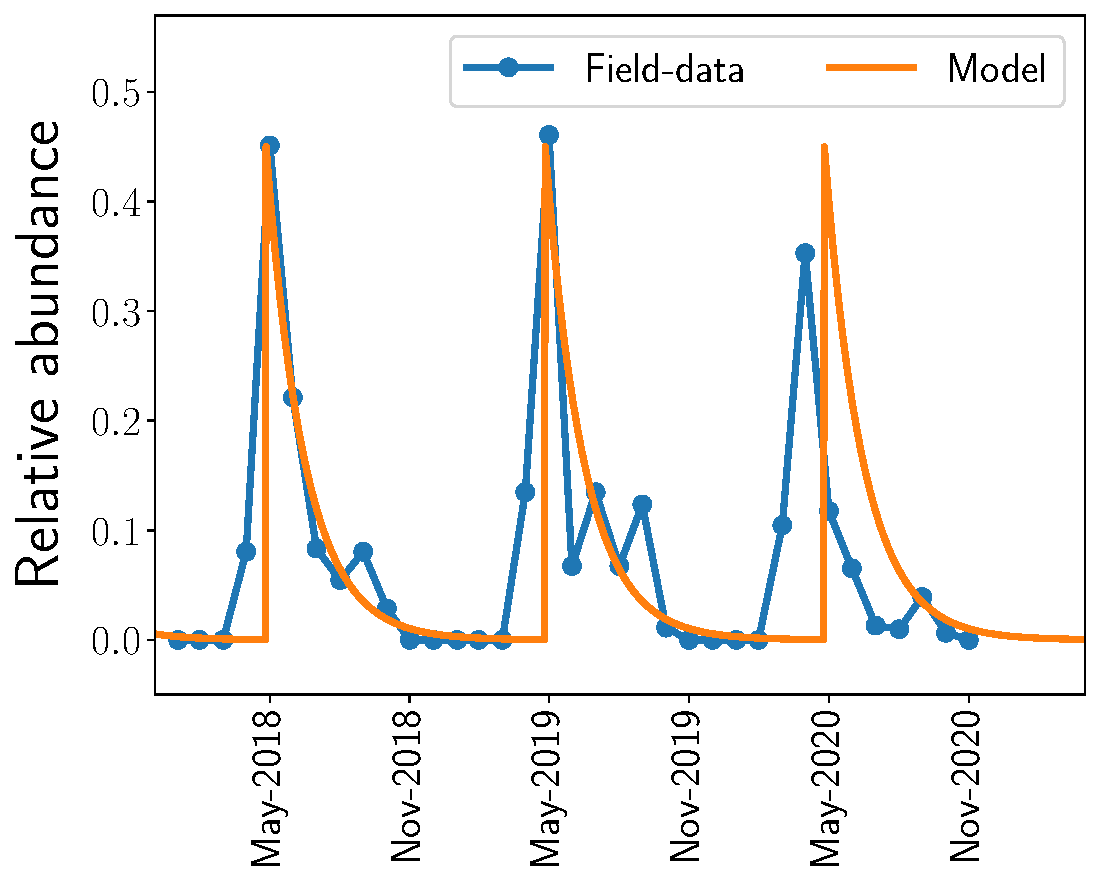
\includegraphics[width=0.85\textwidth]{Figures/Vector_dynamics.pdf}
    \caption[Vector dynamics produced by the model compared to
        field-data]{Vector dynamics produced by the model compared to
        field-data
        from \cite{Lopez2021}.}
    \label{fig:vector_dynamics}
\end{figure}

\cref{fig:vector_dynamics} shows a time series
for the population of \textit{Philaenus spumarius} in Mallorca, taken from
\cite{Lopez2021} (in blue). Superimposed (in orange) is the assumption used in
our model \cref{eq:SEIR_v}, the $\delta(t-nT)$, i.e., every year susceptible
vectors appear in the system.

In our model (\cref{eq:SEIR_v}), the crossed nonlinear terms in $\dot{S}_H$
and $\dot{S}_v$, $S_H I_v$ and $S_v I_H$, are divided by the total host
population, $N_H$. Thus, the vector-to-plant infection process is modeled using
mass action incidence, which is density dependent, while the plant-to-vector
infection process is modeled using standard incidence, which is frequency
dependent \cite{MartchevaBook}. This implies that doubling the number of
vectors in the crop field would double the number of resulting exposed (or
infected) hosts, as this process is population-dependent (mass action
incidence), while doubling the number of hosts would not result in more vectors
per unit area being infected, as this process only depends on the contact
probability, being frequency dependent (standard incidence). We think this is
the most reasonable assumption because, for a given plantation framework,
increasing the number of hosts is expected to also increase the area of the
field, while the number of vectors is an independent quantity.

\subsection{Basic reproductive number}

The basic reproductive number, $R_0$, of the model cannot be trivially
computed using standard methods such as the Next Generation Matrix (NGM)
\cite{Diekmann2010}, as there is no pre-pandemic fixed point in the system of
differential equations \cref{eq:SEIR_v}. For periodically varying vector
populations, rigorous methods have been developed \cite{Bacaer2007}, but not
for the case of growing or decaying vector populations. Here we use the simple
method developed in \cref{ch:xf_PRE} \cite{GimenezRomero2022_PRE} (see
\cref{app:R0}), which
effectively computes the average number of secondary infections produced by an
initially infectious individual in one generation. Thus, the effective basic
reproductive number is given by
\begin{equation}\label{eq:R0}
    R_0=\frac{\beta\alpha}{\mu\gamma}\frac{S_H(0)}{{N_H}^2}
    \frac{N_v(0)}{\mu\tau}\left(1-e^{-\mu\tau}\right)
    \ ,
\end{equation}
where $\tau$ corresponds to the time length of one generation, in our case
one year. This $R_0$ is calculated using the initial susceptible host
population, $S_H(0)$. Below we will also use a time-dependent $R_0(t)$ using
$S_H(t)$.

\subsection{Epidemiological data}

Epidemiological data from an ALSD outbreak in the island of Mallorca,
Balearic Islands, Spain were taken from \cite{Moralejo2020}. Dated phylogenetic
analysis and estimates of disease incidence showed that the introduction of
both subspecies occurred around 1993, with $\sim 79$\% of almond trees infected
by 2017 \cite{Moralejo2020}. The annual proportion of infected individuals in
the almond tree population between 1993 and 2017 was estimated by analyzing
through qPCR the presence of Xf-DNA in the growth rings of $34$ sampled trees
(cf. Fig. 3 in \cite{Moralejo2020}). The disease progression curve was
estimated without distinguishing whether infections were caused by
\textit{multiplex} or \textit{fastidiosa} subspecies. In addition, a two-sided
bootstrap confidence interval for each data point was set using the SciPy
bootstrap function in Python \cite{SciPy}. On the other hand, epidemic data
for OQDS were retrieved from \cite{White2020}. The data consisted of 2 to 3
yearly censuses of symptom prevalence in 17 olive groves infected with Xf
subsp. \textit{pauca} in Apulia, Italy, which were aggregated to fit our model
as shown in Fig. 4 in \cite{White2020}. Because the compartments of our model
are not in one-to-one correspondence with those shown in the work of White et
al. \cite{White2020}, we used the sum of the symptomatic and desiccated
infected trees in the dataset ($I_S+I_D$) to fit the sum of the infected and
dead trees ($I+R$) and the sum of susceptible and asymptomatic hosts ($S+I_A$)
to fit the sum of susceptible and exposed hosts ($S+E$). The processed data
used to fit the model can be found in \cite{CODE}, while the raw data can be
found in the supplementary data accessible online of the cited articles
\cite{Moralejo2020,White2020}.

\subsection{Model fitting through Bayesian Inference}

We employed an informative normal $\mathcal{N}(\hat{\mu},\hat{\sigma}^2)$
prior distribution, with $\hat{\mu}$ and $\sigma$ the mean and standard
deviation, respectively, for previously measured parameters in the literature,
such as the infectious and latent periods for ALSD, $\tau_I\sim\mathcal{N}(14,
    4)$, $\tau_E\sim\mathcal{N}(4, 1)$ \cite{teviotdale2003almond,
    Moralejo2020} and OQDS, $\tau_I\sim\mathcal{N}(3.5, 1)$,
$\tau_E\sim\mathcal{N}(1.75, 0.5)$ \cite{Fierro2019}. The corresponding rates
are given by $\gamma=1/\tau_I$ and $\kappa=1/\tau_E$, respectively. Similarly,
a prior normal distribution was used for the removal rate of vectors,
$\mu\sim\mathcal{N}(0.02, 0.0075)$, as the mean value $\mu=0.02$ already
captures the vector dynamics observed in field data
(\cref{fig:vector_dynamics}). Regarding the prior distribution for
the transmission rates, a very wide and uninformative uniform prior
distribution, $\beta\sim \mathcal{U}(0.001, 1)$ and
$\alpha\sim\mathcal{U}(0.001, 1)$, was used for each parameter. The number of
hosts, $N_H$, was already provided in the datasets, while, given the lack of
information about the vector population, we assumed $N_v(0)=N_H/2$ for the
initial vector population of each year. However, we tested the robustness of
our results by changing $N_v(0)$.

The posterior distributions of the parameters were approximated using the
Markov Chain Monte Carlo algorithm No U-Turn Sampler (NUTS) with the
recommended target acceptance rate of 65\% \cite{Homan2014}. To ensure
proper convergence, we constructed three independent Markov chains with $10^5$
iterations each after a burn-in of $10^4$ iterations and checked that the
results were statistically equivalent. For each chain, we started at the
maximum-likelihood parameters yielded by the Nelder-Mead algorithm with 1000
iterations.

The parameters of our compartmental model were determined by fitting the
model to data by means of a Bayesian Inference framework using the Turing.jl
package \cite{Turing.jl} in Julia \cite{julia}. The scripts used to fit the
model can be found in \cite{CODE}.

\subsection{Sensitivity Analysis}

We performed a Global Sensitivity Analysis (GSA)
\cite{Sensitivity_analysis_book} of the model to assess the relative
contribution of its parameters and their interactions with different features
of the epidemic. In contrast to the Local Sensitivity Analysis (LSA), the GSA
assesses the influence of a large domain of the parameter space on the desired
outputs of the model. We performed GSA by means of a variance-based analysis,
the Sobol method \cite{SOBOL2001271}. This particular method provides
information not only on how a particular parameter alone influences the model
outputs (as happens with LSA), but also due to the nonlinear interactions among
two or more parameters. Briefly, the method considers the model output, $Y$, as
a general function of the inputs, $f(x_1, ..., x_n)$, so that the variance of
the output, $Var(Y)$, is decomposed as the sum of the variances given by the
variations of the parameters alone and its interactions:
$Var(Y)=\sum_{i=1}^nVar(f(x_i)) + \sum_{i<j}^nVar(f(x_i, x_j)) + \cdots$. This
information is organized in what are known as Sobol indices. The total order
indices are a measure of the total variance of the output quantity caused by
variations of the input parameter and its interactions,
$S_T=Var(f(x_1,...,x_n))/Var(Y)$. First-order (or ``main effect'') indices are
a measure of the contribution to the output variance given by the variation of
the parameter alone, but averaged over the variations in other input
parameters, $S_i=Var(f(x_i))/Var(Y)$. Second-order indices take into account
first-order interactions between parameters, $S_{ij}=Var(f(x_i,x_j)) / Var(Y)$.
Further indices can be obtained, describing the influence of higher-order
interactions between parameters, but these are not going to be considered.

Following the Sobol method, we analyzed the variation of the time at which
the infectious population peaks, $t_{peak}$, the magnitude of this peak,
$I_{peak}$, and the final number of dead hosts, $R_{\infty}$, relative to
variations of the model parameters. The method was implemented within the Julia
high-level programming language \cite{julia} using the sub-package
DiffEqSensitivity.jl in the DifferentialEquations.jl package
\cite{DifferentialEquations.jl}.

\newpage
\section{Results}

\subsection{Model fit and parameter estimates}

The posterior distributions of the fitted parameters, including their
estimated mean and median for ALSD and OQDS, are shown in
\cref{fig:parameter_estimates_ALSD,fig:parameter_estimates_OQDS}, respectively,
together with the assumed prior distributions. We observe that the
literature-driven priors for the latent and infectious period, $\tau_E$ and
$\tau_I$, were already very good guesses and changed slightly converging to the
appropriate distribution that better fitted the epidemic data for both ALSD and
OQDS (\cref{fig:parameter_estimates_ALSD}~\textcolor{ref_color}{(A-B)} and
\cref{fig:parameter_estimates_OQDS}~\textcolor{ref_color}{(A-B)}). Similarly,
the prior for the vector
removal rate, $\mu$, obtained from field data, was good enough so that little
changes were needed for convergence
(\cref{fig:parameter_estimates_ALSD}~\textcolor{ref_color}{(C)}
and
\cref{fig:parameter_estimates_OQDS}~\textcolor{ref_color}{(C)}). On the other
hand, we also observe
that the completely uninformative priors for the transmission rates
successfully converged to the posterior distributions
(\cref{fig:parameter_estimates_ALSD}~\textcolor{ref_color}{(D-E)} and
\cref{fig:parameter_estimates_OQDS}~\textcolor{ref_color}{(D-E)}).

\begin{figure}[H]
    \centering
    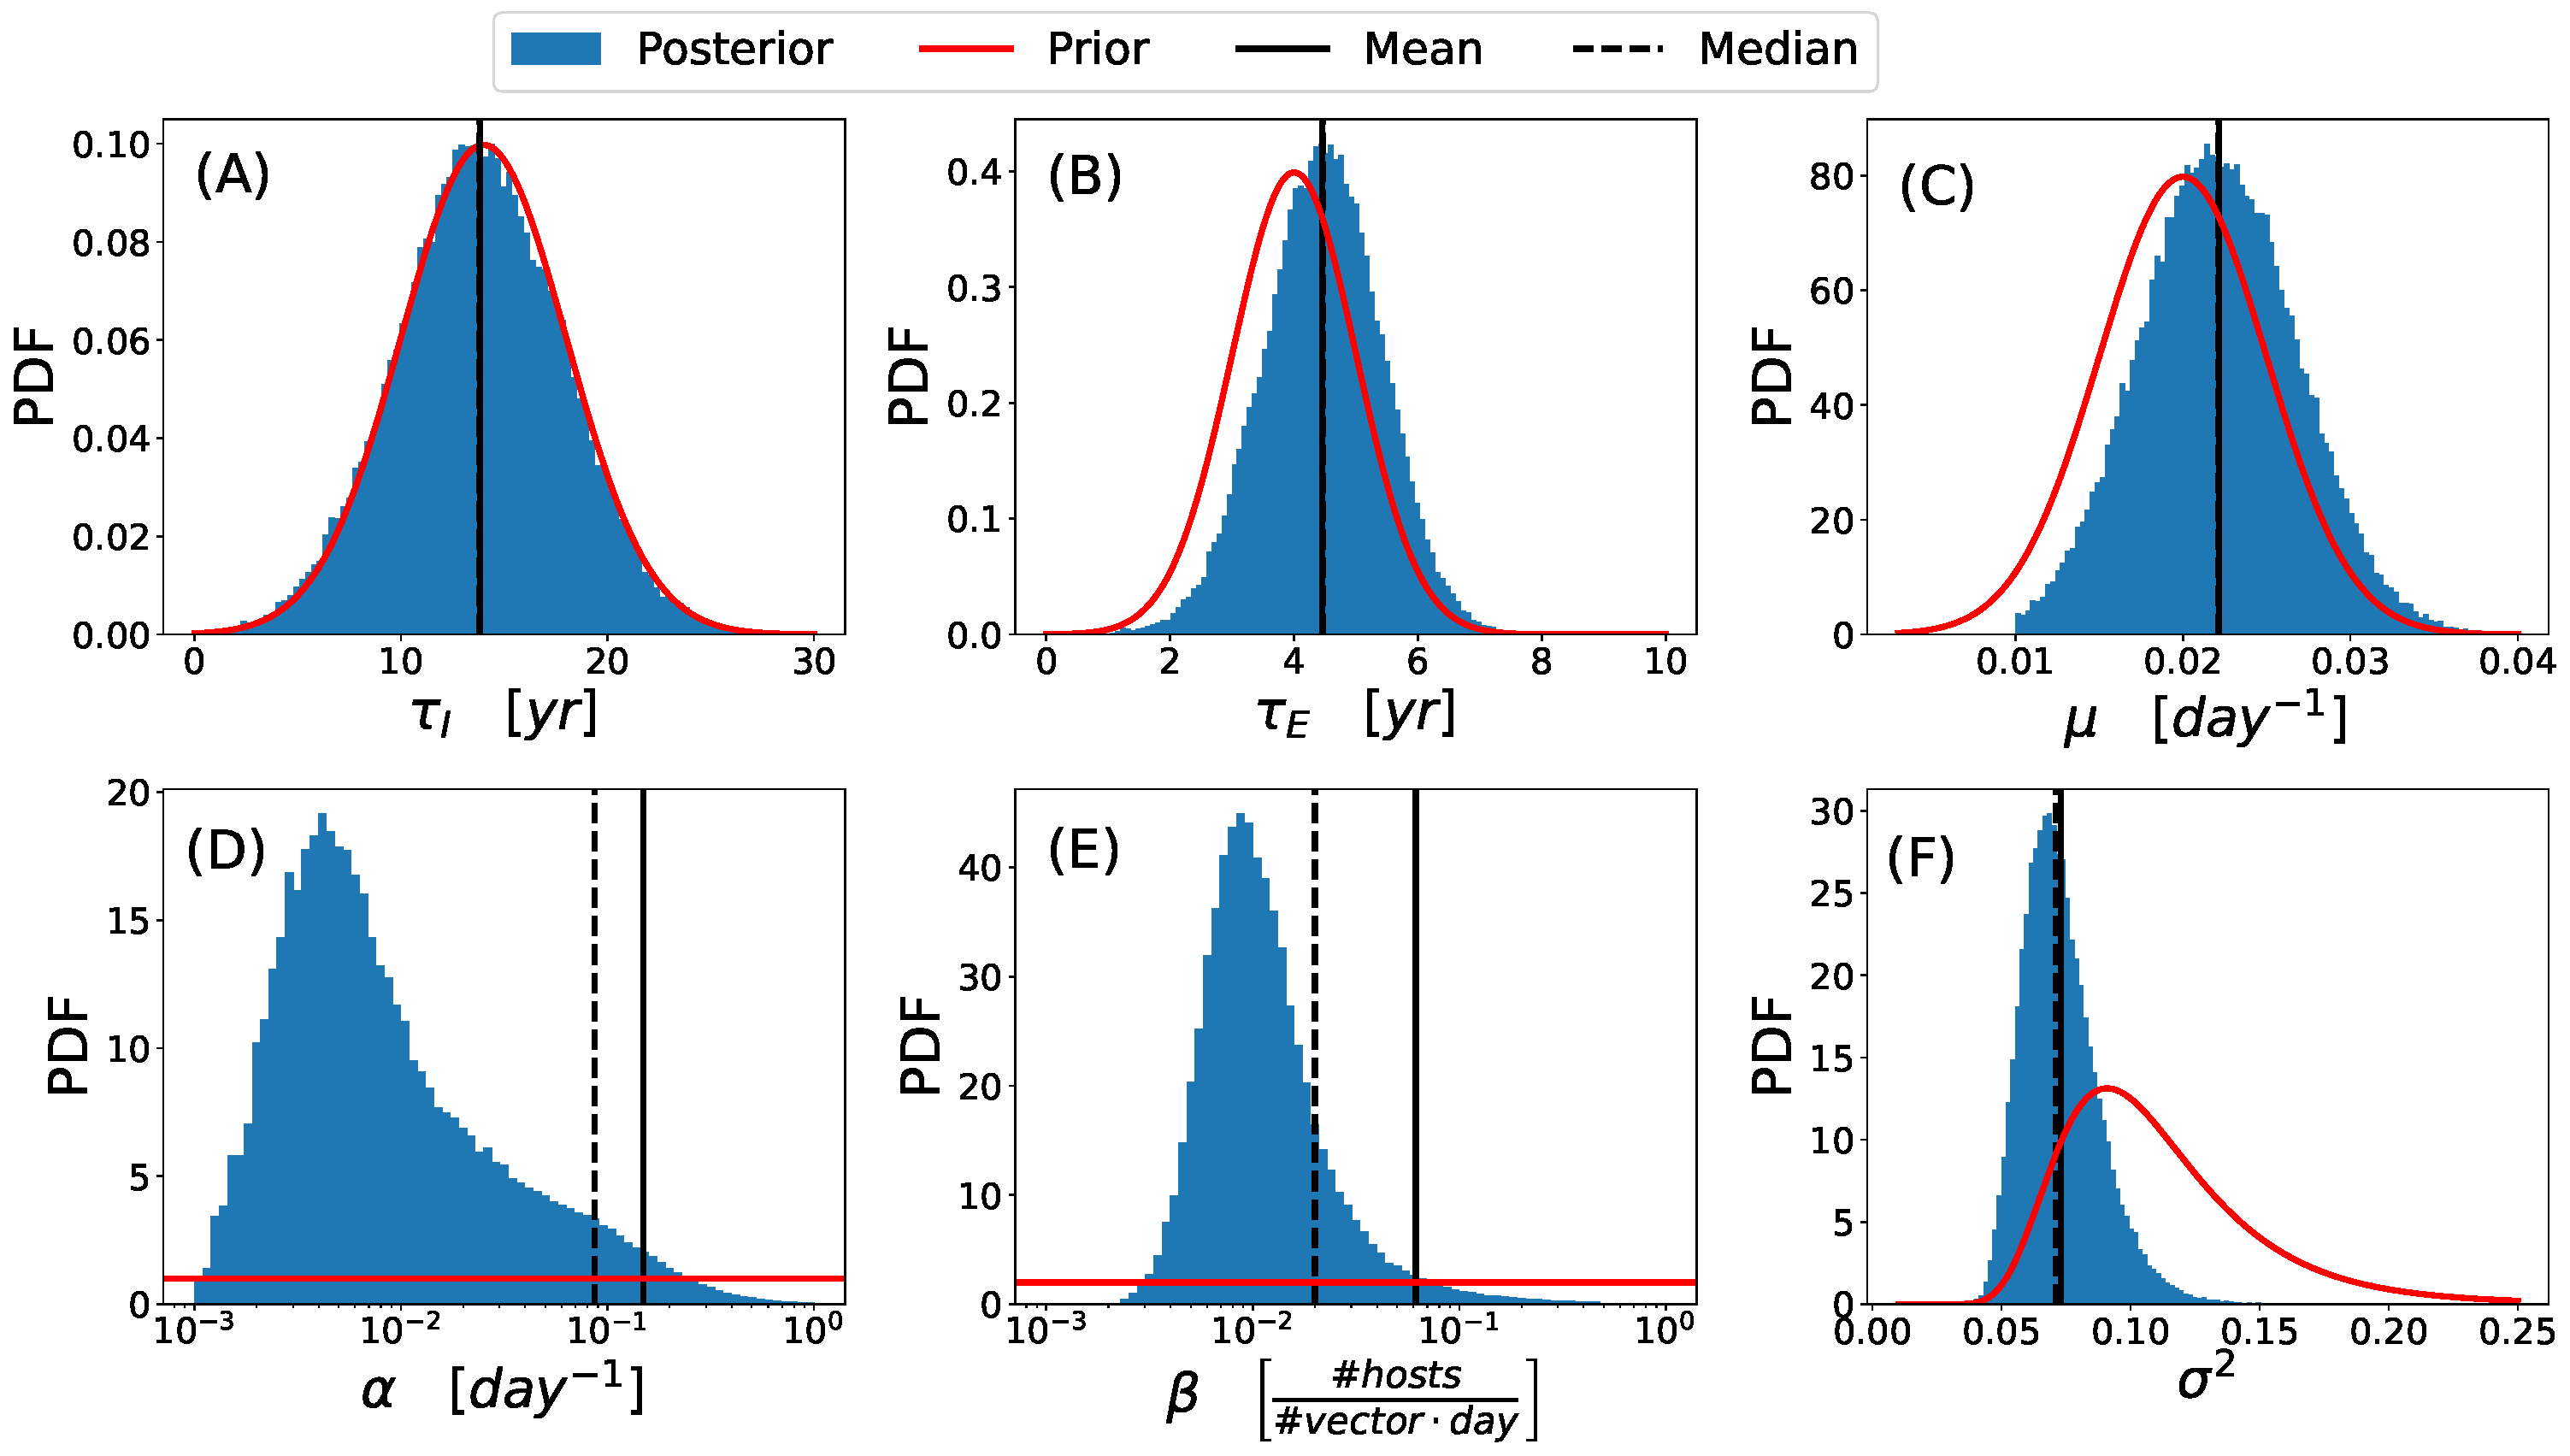
\includegraphics[width=1\textwidth]{Figures/Parameter_estimates_ALSD.pdf}
    \caption[Posterior and prior distributions of the model parameters for
        ALSD]{Posterior (blue histograms) and prior (red line) distributions
        of the model parameters for ALSD. Solid and dashed black lines
        correspond to
        the mean and median of the posterior distributions. (A) Host infectious
        period
        $\tau_I=1/\gamma$. (B) Host latent period $\tau_E=1/\kappa$.  (C)
        Vector
        removal rate $\mu$. (D) Vector infection rate $\alpha$. (E) Host
        infection rate
        $\beta$. (F) The variance of the field data $\sigma^2$.}
    \label{fig:parameter_estimates_ALSD}
\end{figure}

The latter distributions are far from a Gaussian-like shape (note that the
x-axis is log-scaled), being heavy-tailed. This kind of distribution highly
distorts the statistical measures of mean, median, and standard error,
indicating that the estimates for transmission rates are not as robust as the
estimates for the other parameters. These rather uninformative distributions
are most probably arising because of the lack of data about the vector, i.e.,
$S_v(t)$ and $I_v(t)$, to constrain the fits. In essence, many combinations of
$\alpha$ and $\beta$ can similarly fit the host data while yielding quite
different time series for $S_v(t)$ and $I_v(t)$, which cannot be contrasted due
to the lack of field data. Nevertheless, the obtained best-fit mean and median
parameters, although quite different, are able to perfectly fit the data
(\cref{fig:best_fit_model}). Finally, we also observe that the variance for the
field data also converged to a bell-shaped distribution.

\begin{figure}[H]
    \centering
    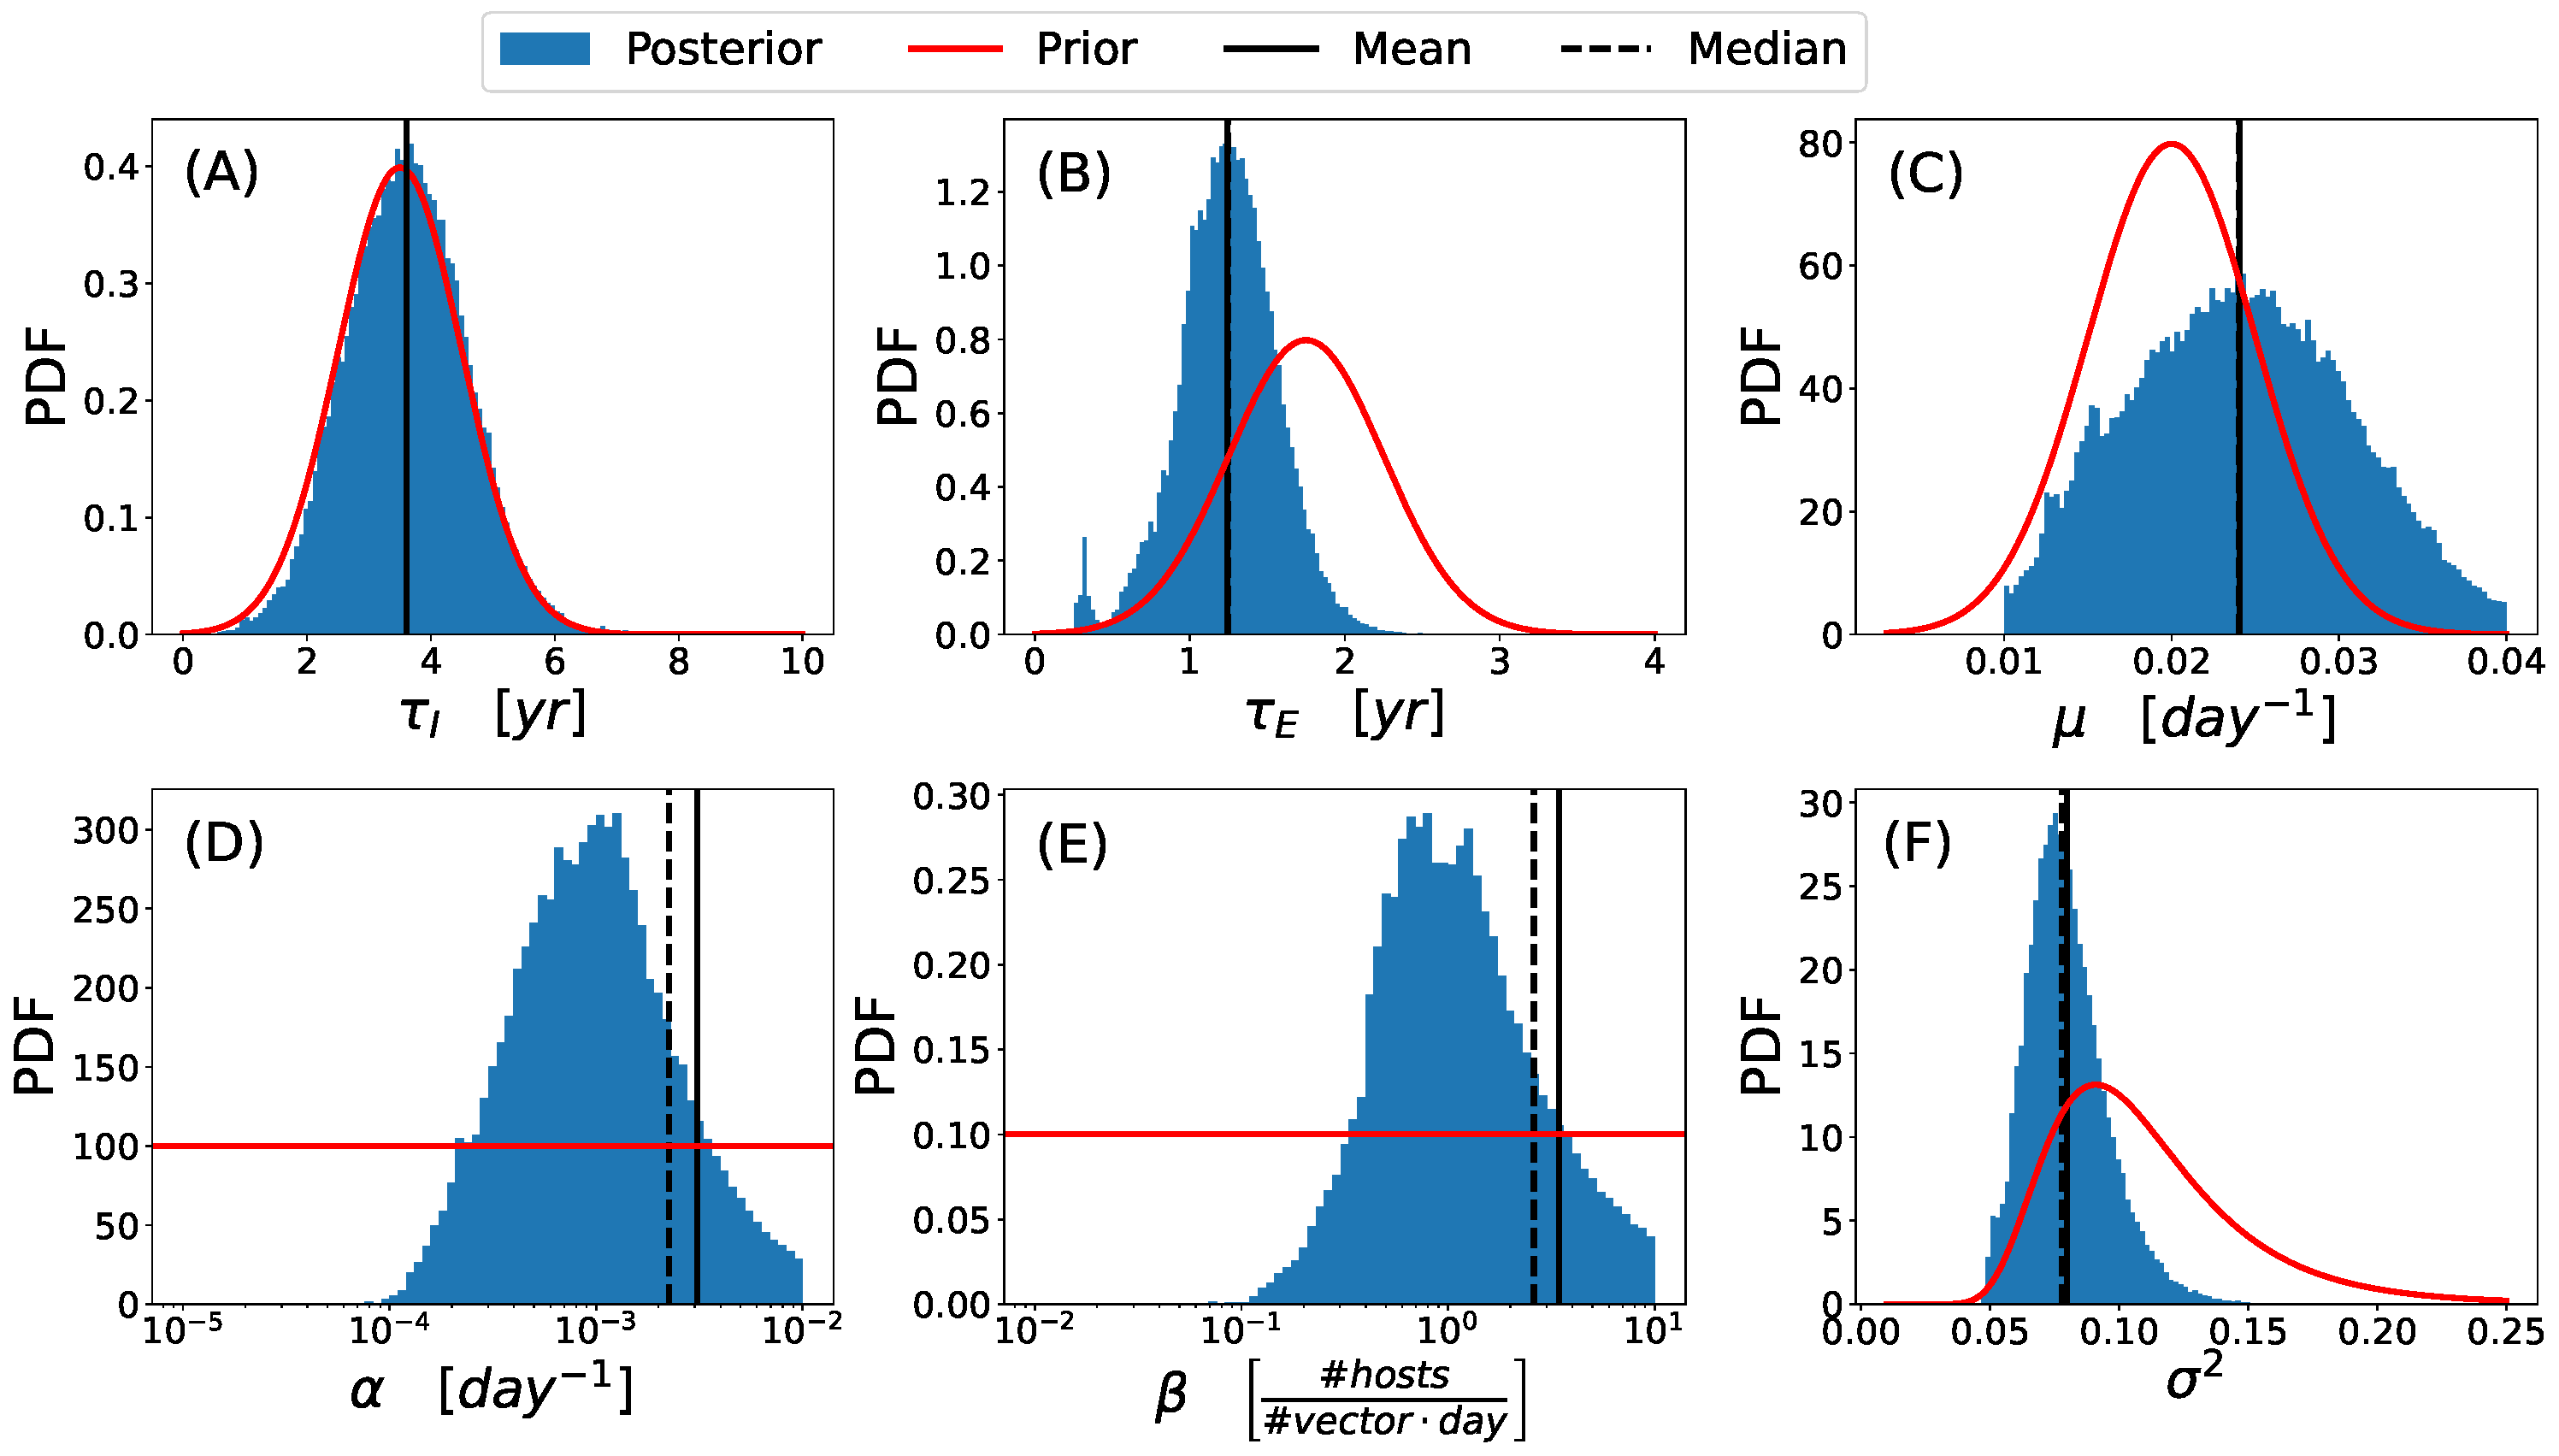
\includegraphics[width=1\textwidth]{Figures/Parameter_estimates_OQDS.pdf}
    \caption[Posterior and prior distributions of the model parameters for
        OQDS]{Posterior (blue histograms) and prior (red line) distributions
        of the model parameters for OQDS. Solid and dashed black lines
        correspond to
        the mean and median of the posterior distributions. (A) Host infectious
        period
        $\tau_I=1/\gamma$. (B) Host latent period $\tau_E=1/\kappa$. (C) Vector
        removal
        rate $\mu$. (D) Vector infection rate $\alpha$. (E) Host infection rate
        $\beta$. (F) Variance of the field data $\sigma^2$.}
    \label{fig:parameter_estimates_OQDS}
\end{figure}

Mean and median parameter estimates, i.e., the best-fit parameter values for
ALSD and OQDS, are summarized in
\cref{tab:parameter_estimates_ALSD,tab:parameter_estimates_OQDS}, respectively.
As already seen from the posterior distributions, the best-fit values for
$\tau_E$, $\tau_I$, and $\mu$ are close to the ones given by literature and
field data for both diseases. Conversely, $\alpha$ and $\beta$ are rather
uninformative, as their 95\% confidence intervals cover almost two orders of
magnitude. This again indicates that without some data about the evolution of
the vector states in time, $S_v(t)$ and $I_v(t)$, it is nearly impossible to
derive the proper values for these parameters.

\begin{table}[H]
    \centering
    \caption[Estimated parameters of the model for ALSD in Mallorca]{Estimated
        epidemiological
        parameters from Bayesian model
        fitting to the disease progression curve of ALSD in Mallorca.}
    \resizebox{\textwidth}{!}{
        \begin{tabular}{cccccc}
            \hline \hline
            \textbf{Parameter}      & \textbf{Definition}       &
            \textbf{Units}          &
            \textbf{Posterior Mean} & \textbf{Posterior Median} & \textbf{95\%
                C.I.}
            \\
            \hline
            $\tau_I$                & Host infectious period    & yr
                                    & $13.84$                   & $13.82$
                                    &
            $[7.12, 20.47]$
            \\
            $\tau_E$                & Host latent period        & yr
                                    & $4.46$                    & $4.47$
                                    & $[2.88,
                        5.99]$
            \\
            $\beta$                 & Host infection rate       &
            $\SI{}{\frac{\#host}{\#vector
            \cdot day}}$            & $0.062$                   & $0.02$
                                    & $[0.0061, 0.3013]$
            \\
            $\alpha$                & Vector infection rate     &
            $\SI{}{day^{-1}}$       & $0.15$                    &
            $0.086$                 & $[0.0047, 0.54]$
            \\
            $\mu$                   & Vector removal rate       &
            $\SI{}{day^{-1}}$       & $0.0222$                  &
            $0.0221$                & $[0.015, 0.030]$
            \\
            $R_0$                   & Basic reproductive number & -
                                    & 133                       & 25
                                    & -
            \\ \hline
            \hline
        \end{tabular}
    }
    \label{tab:parameter_estimates_ALSD}
\end{table}

Overall, the data falls within the 99\% confidence limits of the fitted
model for both the ALSD and OQDS outbreaks
(\cref{fig:best_fit_model}~\textcolor{ref_color}{(B, D)}).
We
also computed the instantaneous reproductive number, $R_0(t)$, by using
\cref{eq:R0} with $S_H(t)$ instead of only $S_H(0)$ along the simulation.
Noteworthy, $R_0(t)=1$ coincides with the stopping of new infections being
produced, i.e., the number of exposed hosts does not increase
(\cref{fig:best_fit_model}~\textcolor{ref_color}{(A, C)}). This supports our
approximate method for
computing the reproductive number for Xf diseases (\cref{app:R0},
\cref{eq:R0}). Due to the different time scales of both epidemics
($\tau_I^{ALSD}+\tau_E^{ALSD} > \tau_I^{OQDS}+\tau_E^{OQDS}$), the OQDS
outbreak dies out earlier than the one for ALSD.

\begin{table}[H]
    \centering
    \caption[Estimated parameters of the model for OQDS in Apulia]{Estimated
        epidemiological parameters from Bayesian model
        fitting to the disease progression curve of OQDS in Apulia.}
    \resizebox{\textwidth}{!}{%
        \begin{tabular}{cccccc}
            \hline \hline
            \textbf{Parameter}      & \textbf{Definition}       &
            \textbf{Units}          &
            \textbf{Posterior Mean} & \textbf{Posterior Median} & \textbf{95\%
                C.I.}
            \\
            \hline
            $\tau_I$                & Host infectious period    & yr
                                    & $3.61$                    & $3.60$
                                    & $[2.06,
                        5.20]$
            \\
            $\tau_E$                & Host latent period        & yr
                                    & $1.24$                    & $1.25$
                                    & $[0.70,
                        1.75]$
            \\
            $\beta$                 & Host infection rate       &
            $\SI{}{\frac{\#host}{\#vector
            \cdot day}}$            & $3.44$                    & $2.60$
                                    & $[0.55, 8.79]$
            \\
            $\alpha$                & Vector infection rate     &
            $\SI{}{day^{-1}}$       & $0.0031$                  &
            $0.0022$                & $[0.0005, 0.0084]$
            \\
            $\mu$                   & Vector removal rate       &
            $\SI{}{day^{-1}}$       & $0.0240$                  &
            $0.0240$                & $[0.014, 0.035]$
            \\
            $R_0$                   & Basic reproductive number & -
                                    & 33                        & 21
                                    & -
            \\ \hline
            \hline
        \end{tabular}
    }
    \label{tab:parameter_estimates_OQDS}
\end{table}

We notice that for ALSD a large proportion of the vector population gets
infected every year (\cref{fig:best_fit_model}~\textcolor{ref_color}{(A)}),
while a very small
proportion is needed in OQDS to produce a lethal outbreak
(\cref{fig:best_fit_model}~\textcolor{ref_color}{(C)}). However, this last
statement is rather
unrealistic, as around 50\% of the vectors that are captured in Apulia are
indeed infected by Xf \cite{Cavalieri2019,cornara2017transmission}. Thus, the
evolution of the infected vector population should be qualitatively similar to
that obtained for ALSD (\cref{fig:best_fit_model}~\textcolor{ref_color}{(C)}).
As previously
explained,
different suitable combinations of $\alpha$ and $\beta$ parameters should give
rise to similar progression curves for the hosts while different ones for the
vectors, but the realistic values for these parameters cannot be obtained from
the Bayesian fit due to the lack of data of the vector states, $S_v(t)$, and
$I_v(t)$.

\begin{figure}[H]
    \centering
    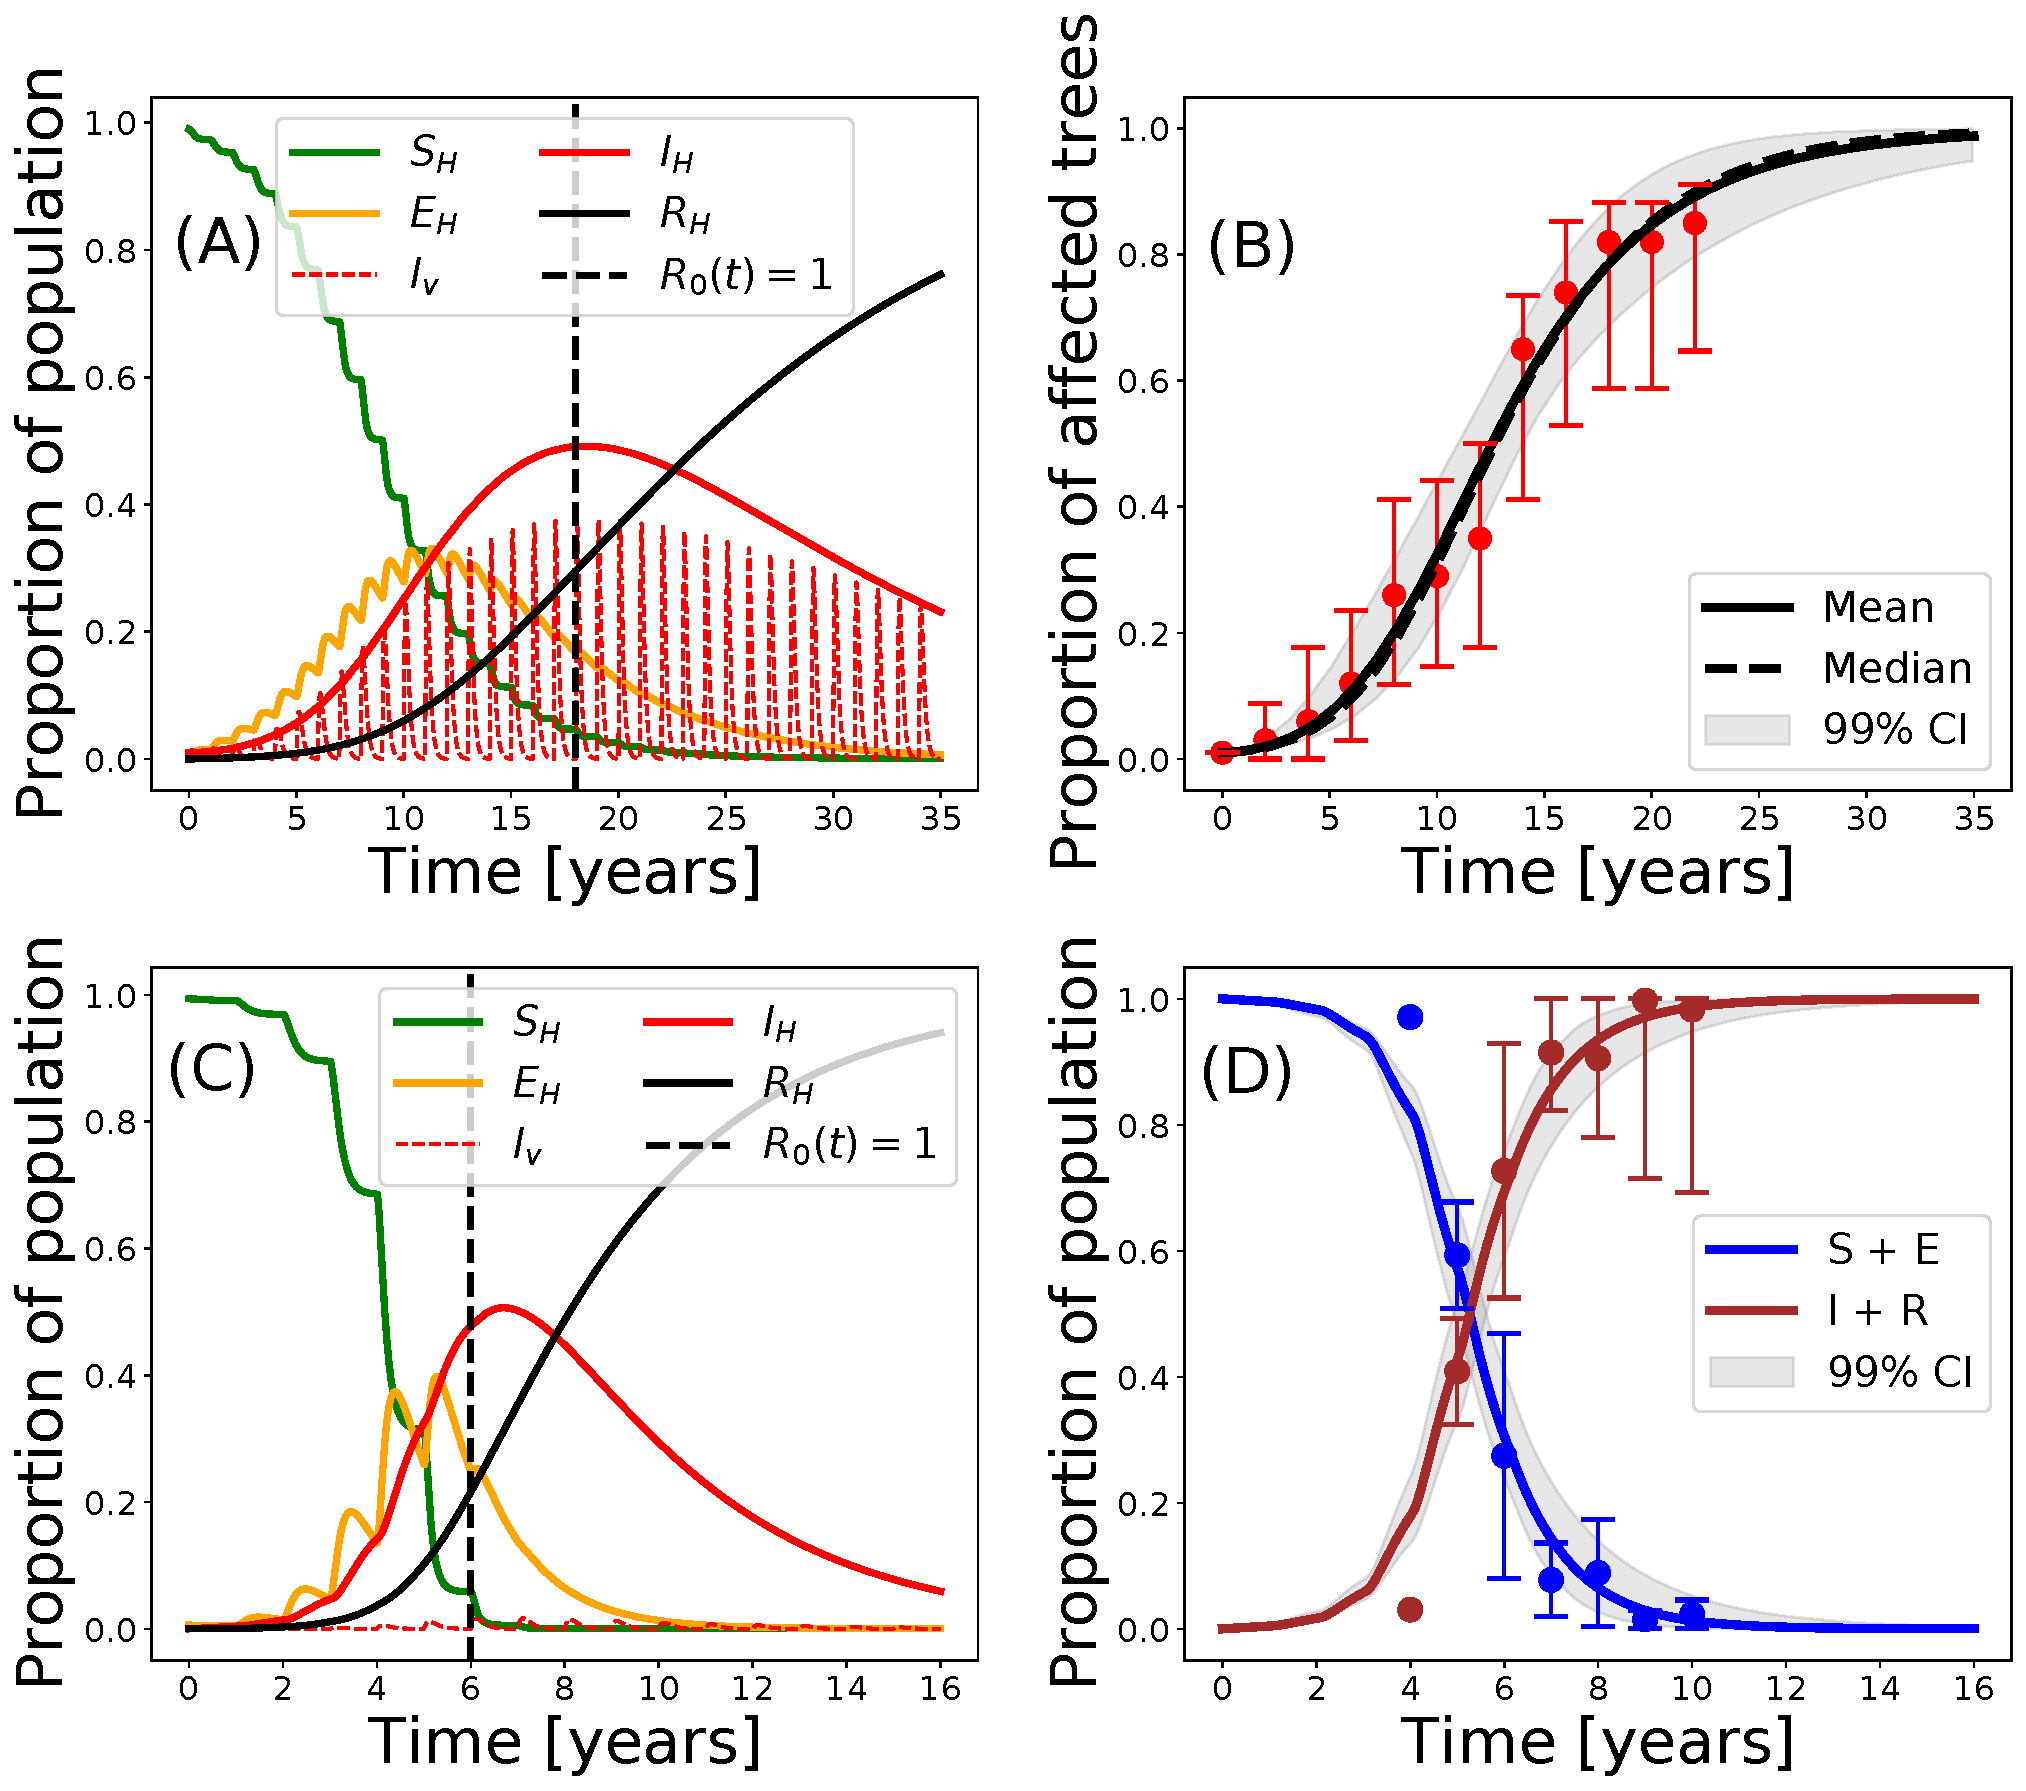
\includegraphics[width=1\textwidth]{Figures/BayesianInference.pdf}
    \caption[Best-fit model to the field data for ALSD and OQDS]{(A) Simulation
        of the model with the best-fit parameters for
        ALSD. (B) Model fit to field data by means of the mean and median
        values of the posterior distributions of the parameters for ALSD. (C)
        Simulation of the model with the best-fit parameters for OQDS. (D)
        Model fit to field data by means of the mean and median values of the
        posterior distributions of the parameters for OQDS. The gray-shaded
        area corresponds to the 99\% confidence interval. The error bars for
        the field data correspond to their 95\% confidence interval obtained
        with a bootstrapping technique.}
    \label{fig:best_fit_model}
\end{figure}

Nevertheless, by manually exploring other values for $\alpha$ and $\beta$
parameters, we can obtain a more biologically plausible scenario for the OQDS
that is still able to fit the available data for the hosts.
\cref{fig:best_fit_model_OQDS}~\textcolor{ref_color}{(A)} shows a simulation of
the model with
previously inferred best-fit median parameters for OQDS. By changing the values
of $\alpha$ and $\beta$, we obtain a more realistic scenario, i.e., around
50\% of the vector population getting infected during the outbreak
(\cref{fig:best_fit_model_OQDS}~\textcolor{ref_color}{(B)})
\cite{Cavalieri2019,
    cornara2017transmission}. Noteworthy, the $\beta$ value obtained in this
way
is almost identical to the transmission rate recently reported by
\cite{Bodino2021} for OQDS. This change in the transmission parameters only
affects the progression curve of the infected vector population, being the
progression of the host compartments practically unchanged
(\cref{fig:best_fit_model_OQDS}~\textcolor{ref_color}{(C)}). Anyway, both sets
of parameter values for
$\alpha$ and $\beta$ can properly fit the field data, corresponding exclusively
to the	host population
(\cref{fig:best_fit_model_OQDS}~\textcolor{ref_color}{(D)}).

The model adjusted to the progression curves of both diseases indicates
that the transmission rate $\alpha$ must be greater than $\beta$ when the
proportion of infected vectors is relatively high ($>30\%$). We checked if the
relation between $\alpha$ and $\beta$ held when changing the assumed
$N_v(0)=N_H/2$, obtaining that it kept approximately the same for very
different values of the initial vector population.

\begin{figure}[H]
    \centering

    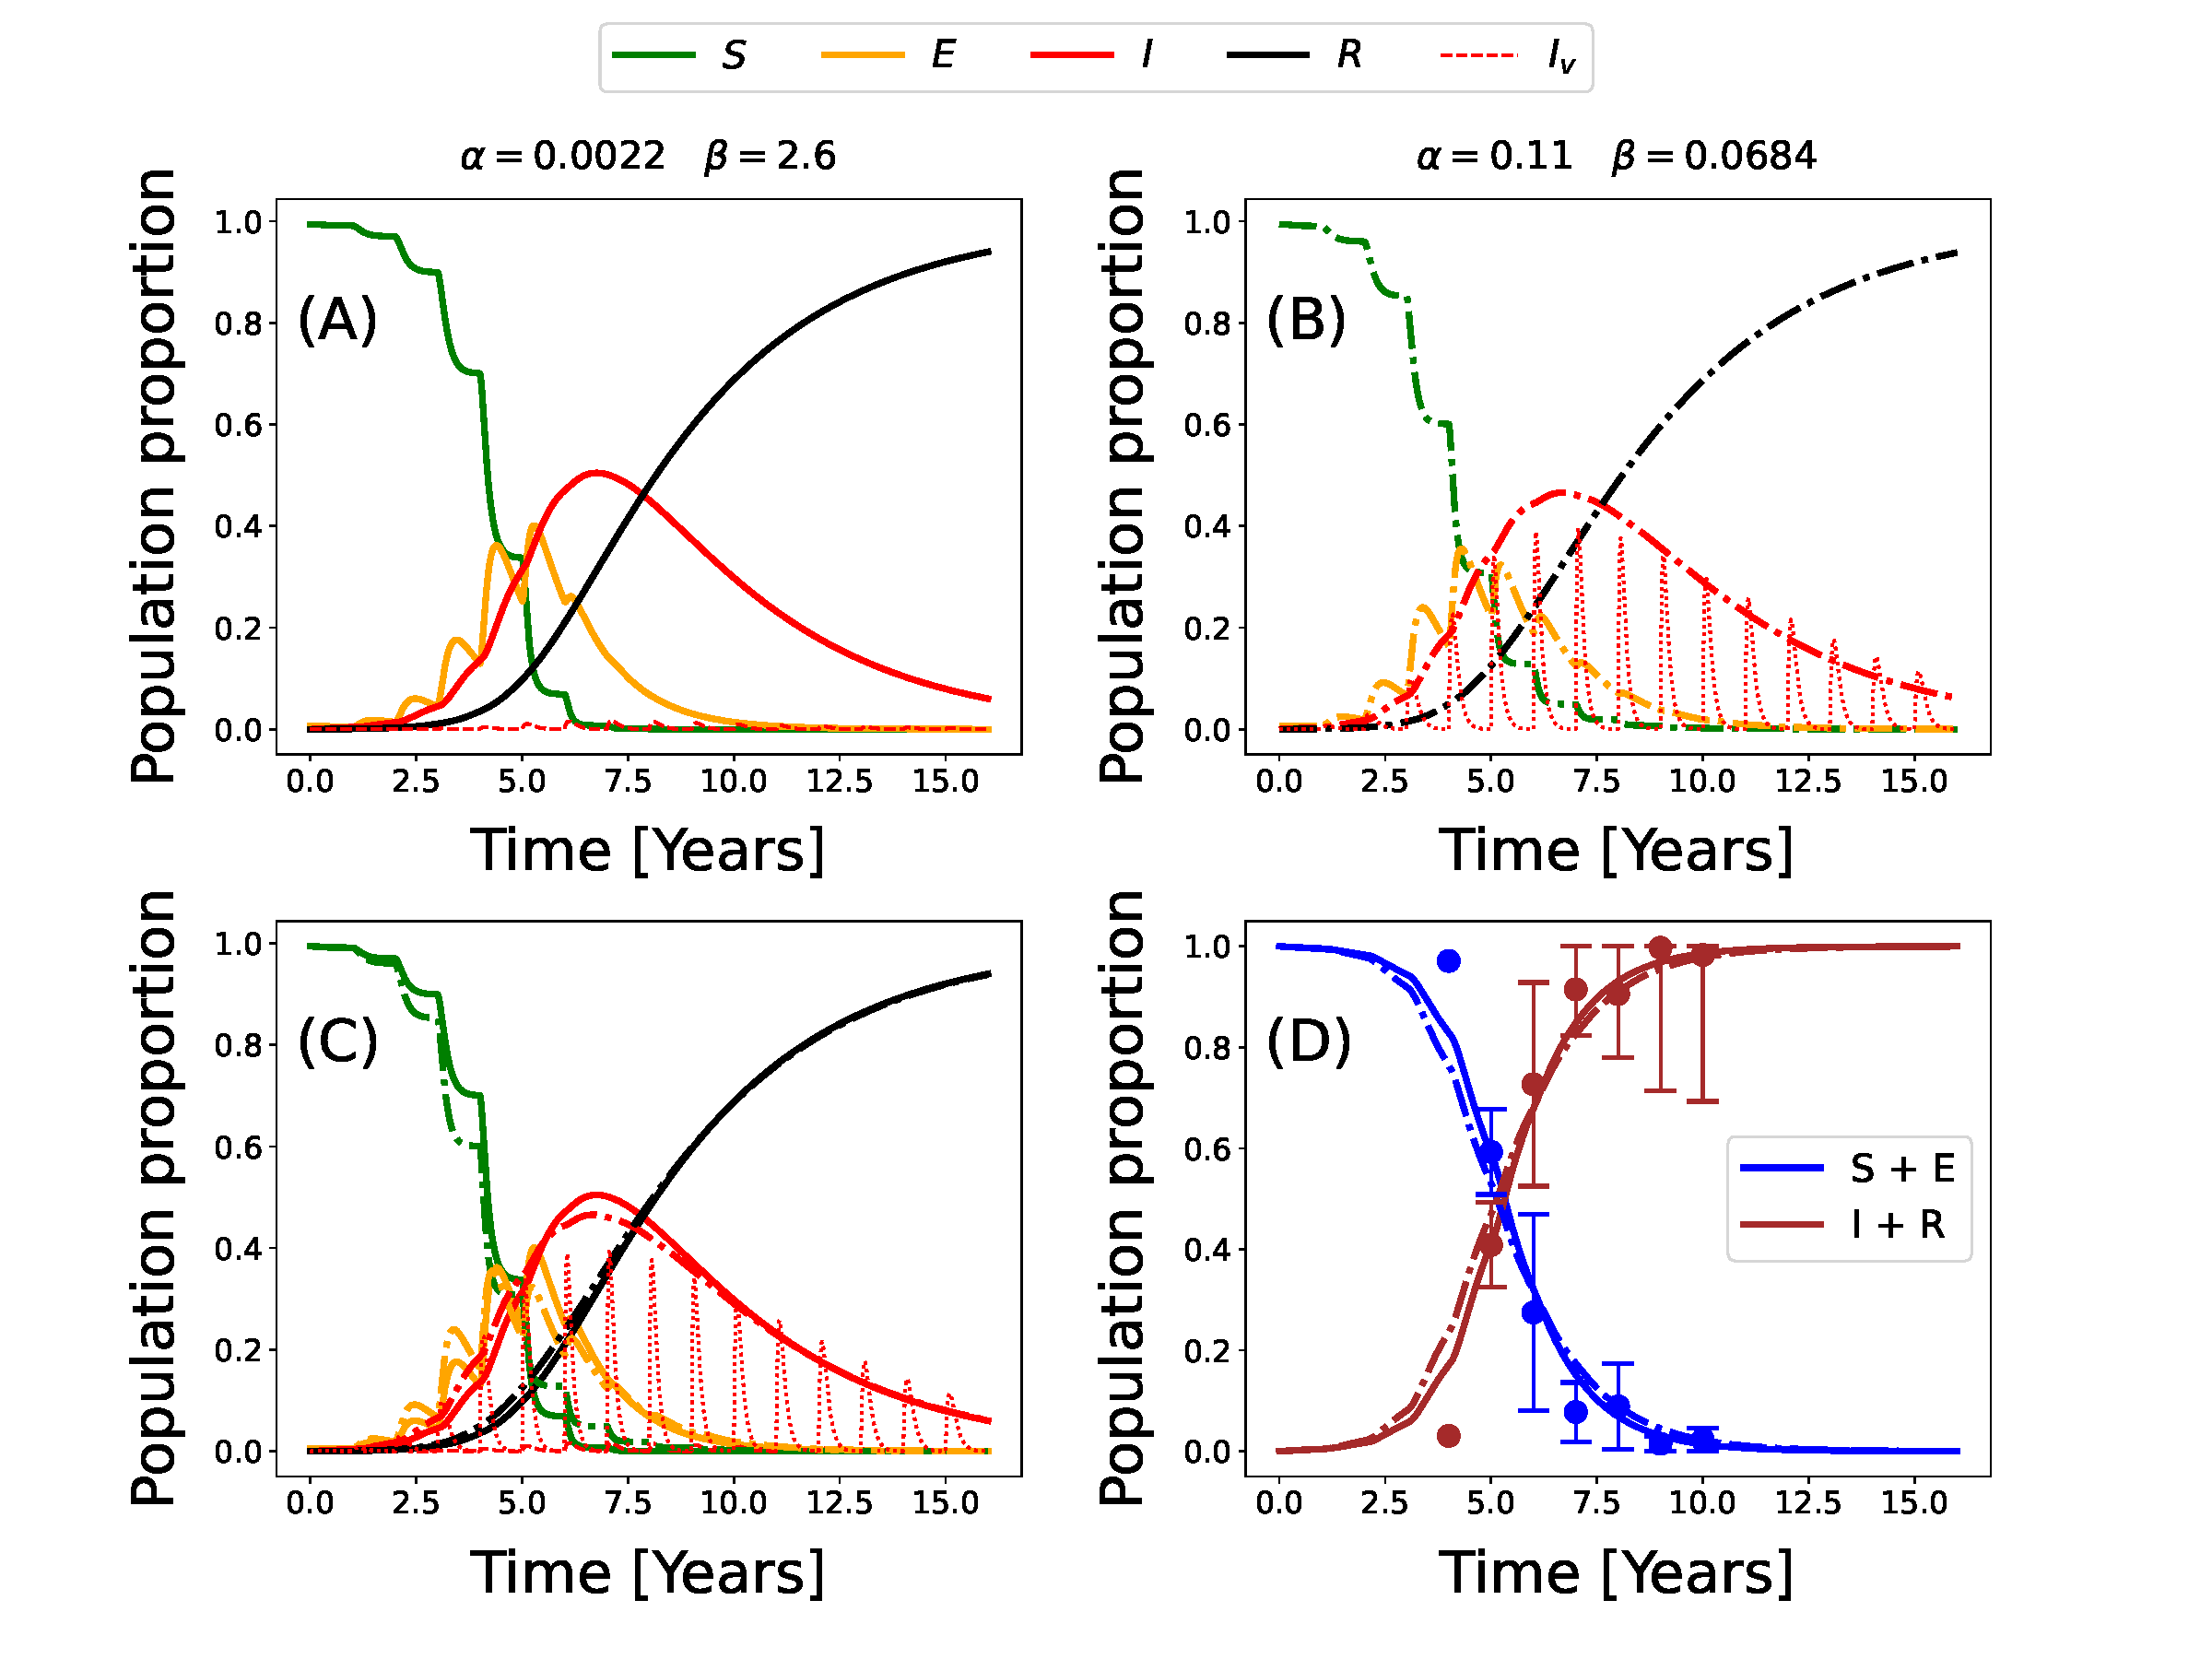
\includegraphics[width=\textwidth]{Figures/OQDS_different_vector_curves_same_host_curve.pdf}
    \caption[Comparison of the model fit to the data for OQDS with different
        transmission rates]{(A) Simulation of the model with the original
        best-fit parameters for OQDS. (B) Simulation of the model with the
        original best-fit parameters for OQDS but with different $\alpha$,
        $\beta$ values. (C) Comparison of the progression curves. Note that the
        curves for the hosts are very similar, while the curve for the infected
        vector population is very different. (D) Comparison of the model fit to
        the data with both simulations. Solid lines correspond to results with
        the original best-fit parameters, while dash-dot lines correspond to
        the	results of the more realistic scenario with different $\alpha$
        and $\beta$.}
    \label{fig:best_fit_model_OQDS}
\end{figure}

\subsection{Global Sensitivity Analysis}

We computed the sensitivity indices for the model parameters with respect
to the more relevant quantities of interest, namely, the time at which the
number of infectious hosts is maximal, $t_{\textrm{peak}}$, the maximum number
of infectious hosts, $I_{\textrm{peak}}$, and the final number of dead hosts,
$R_\infty$. The results were obtained exploring the parameter space constrained
to the intervals $\{\beta\in(0.001, 0.1), \ \tau_E\in(3,7), \ \tau_I\in(5,25),
    \ \alpha\in(0.001, 1), \ \mu\in(0.01, 0.04)\}$ using $10^4$ Quasi-Monte
Carlo
samples and are summarized in \cref{fig:GSA}.

\begin{figure}[H]
    \centering
    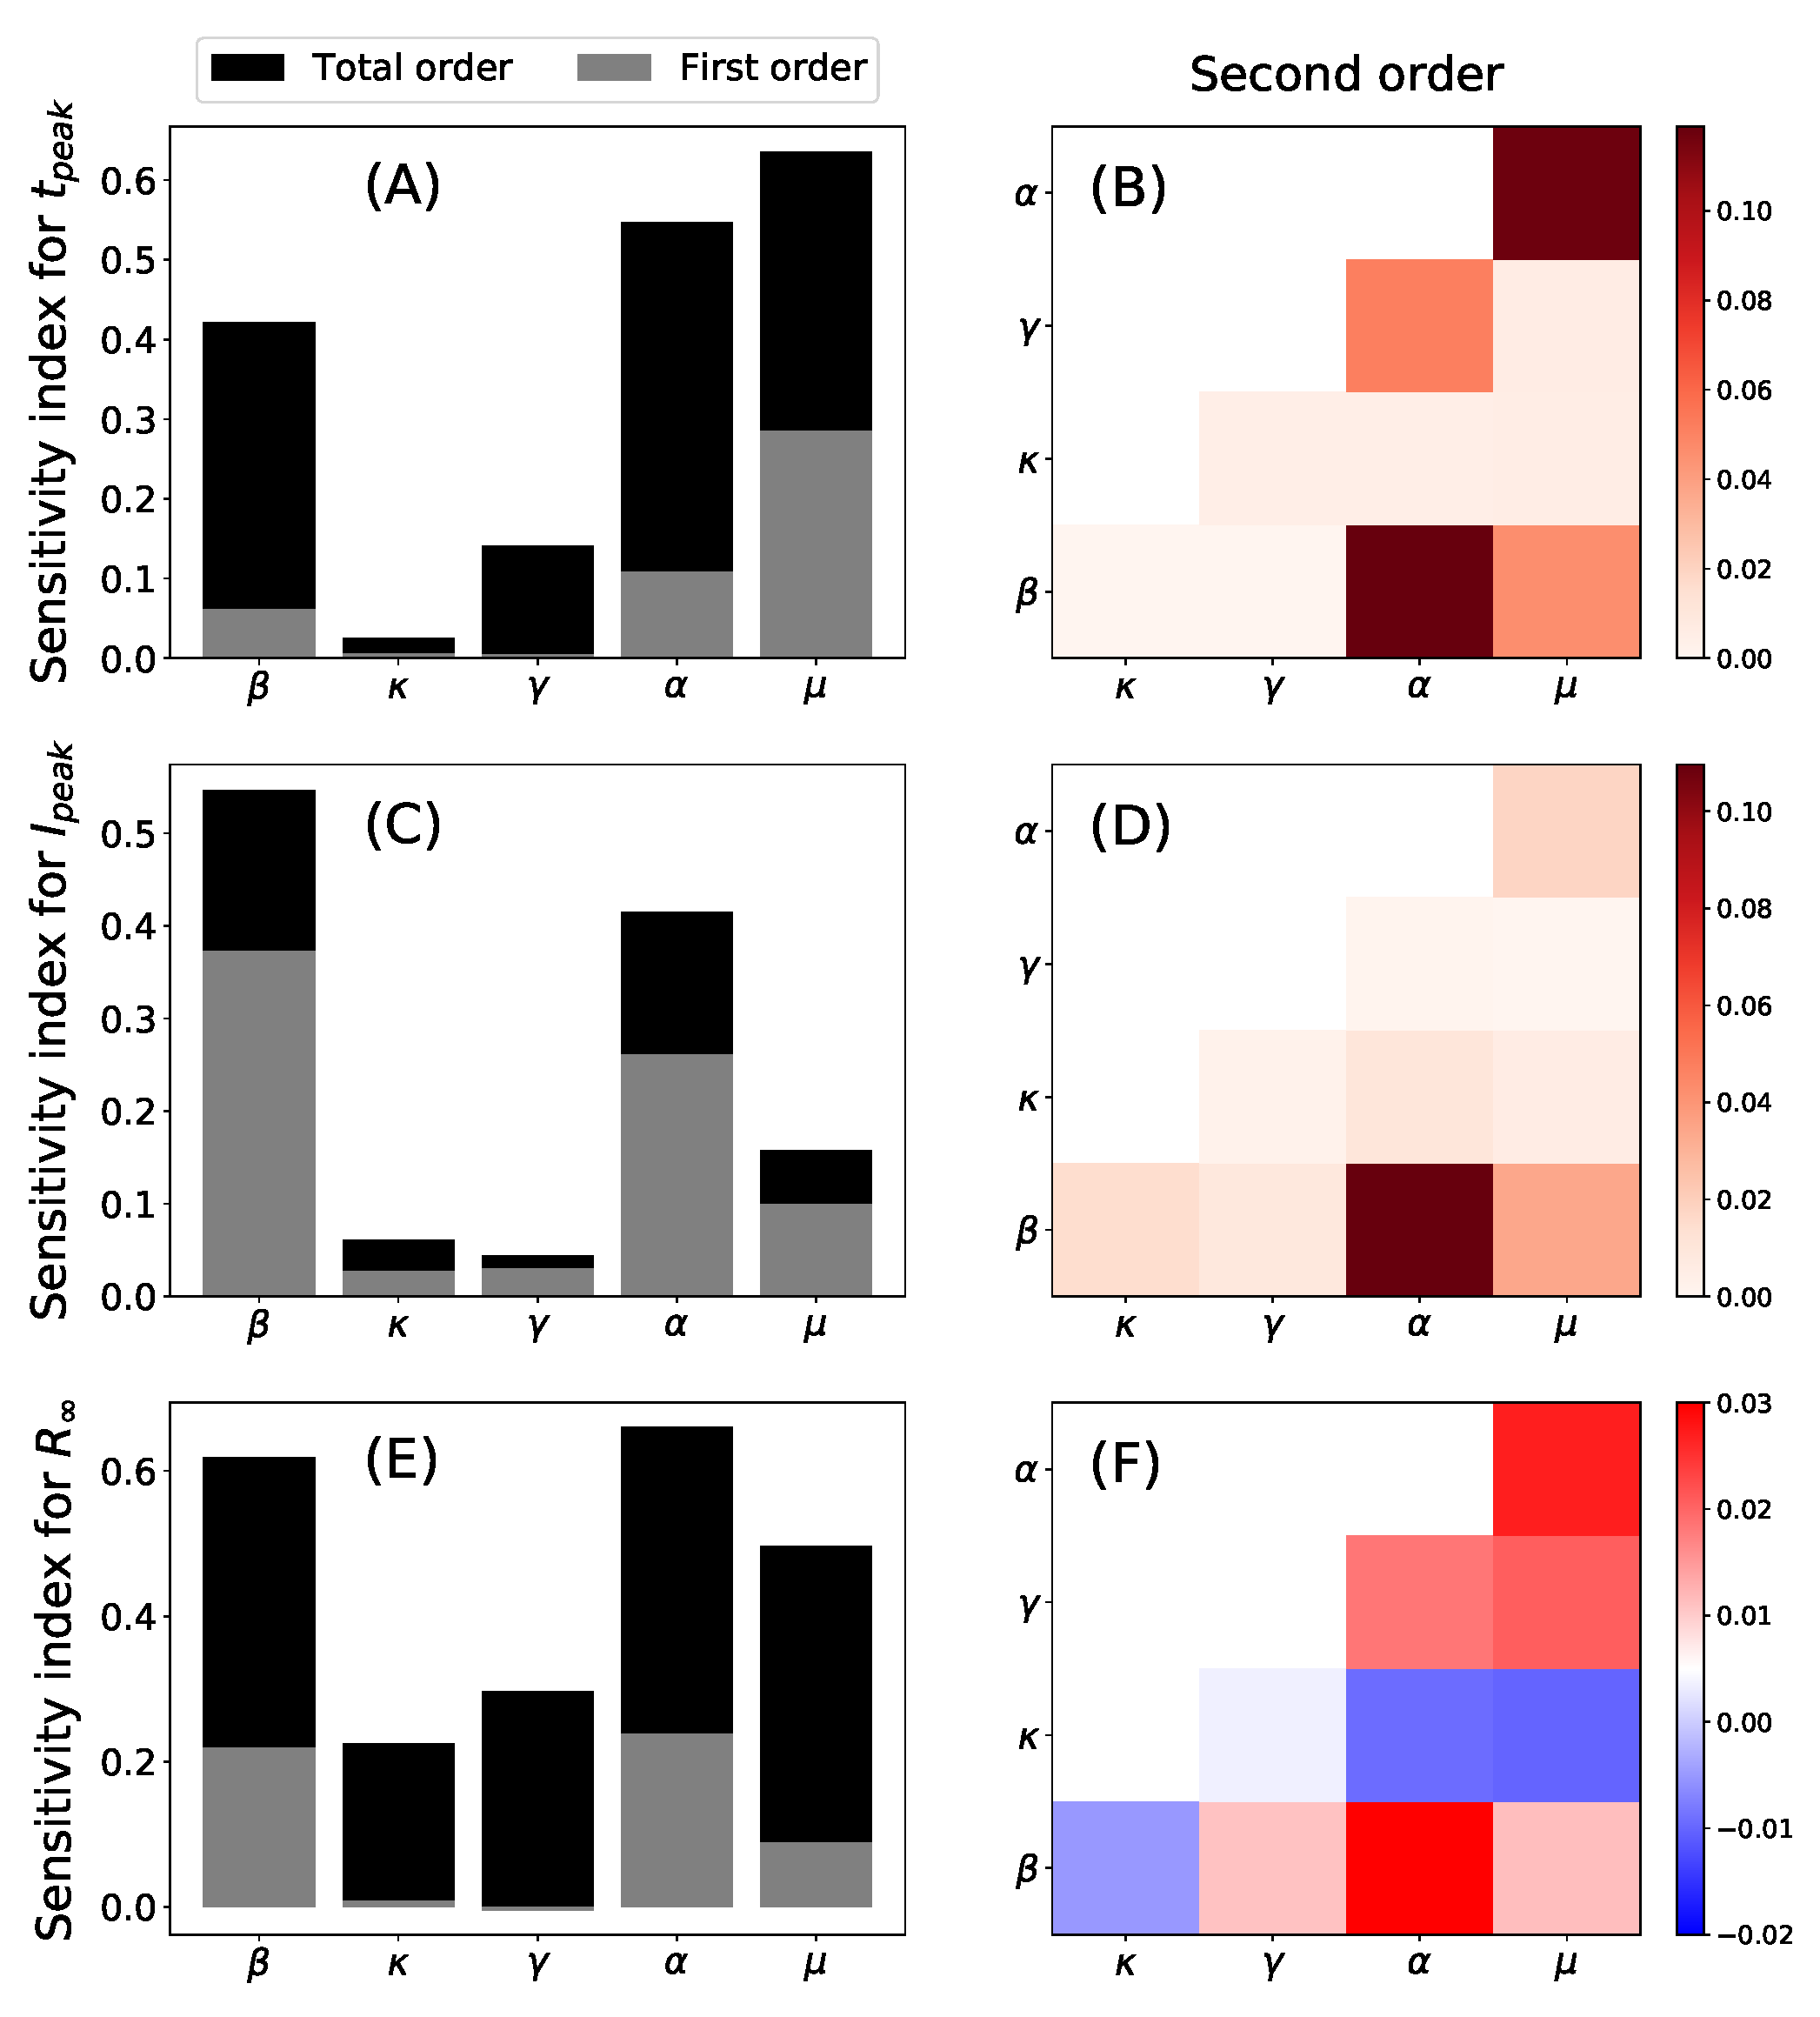
\includegraphics[width=0.85\textwidth]{Figures/GSA.pdf}
    \caption[Global Sensitivity Analysis of the model]{Global Sensitivity
        Analysis of the model parameters performed
        with the Sobol method with respect to the time at which the infectious
        population peaks, $t_{peak}$ (A-B), the magnitude of this peak,
        $I_{peak}$ (C-D), and the final number of dead hosts, $R_{\infty}$
        (E-F). The left column (A,C,E) shows the total and first-order indices
        and the right column (B,D,F) shows the second-order indices.}
    \label{fig:GSA}
\end{figure}

Parameters $\alpha, \ \beta$, and $\mu$ are the most influential with regard
to the time at which the infectious host population peaks, $t_{peak}$, the
magnitude of the peak, $I_{peak}$, and the final number of dead hosts,
$R_{\infty}$. The total output variance (total order indices) cannot be
explained by the variances of the parameters alone (first order indices)
(\cref{fig:GSA}). Therefore, higher-order interactions among the parameters
importantly affect the sensitivity of the quantities under study. Indeed, the
contribution to the total output variance of $\gamma$ and $\kappa$ for
$t_{peak}$ and $R_{\infty}$ come notably from higher-order interactions. This
can be checked in panels (B,C,F) of \cref{fig:GSA}, in which the contribution
to the output variance from interactions between pairs of parameters (second
order indices) is represented. Interactions among the parameters contribute to
increasing the output variance with respect to $t_{peak}$ and $I_{peak}$, while
the effect is more heterogeneous in the case of $R_{\infty}$. In particular,
the interactions between $\alpha-\beta$ and $\alpha-\mu$ produce the main
contributions to the increase of output variance in all cases, while
$\kappa-\beta$, $\kappa-\alpha$, and $\kappa-\mu$ interactions decrease the
output variance.

\subsection{Epidemic control through vector management}

The sensitivity analysis clearly indicates that acting on $\alpha,\beta$,
and $\mu$ is the best strategy to lower disease incidence and mortality.
However, controlling transmission rates is cumbersome, so a different control
strategy based only on vector control is considered in this section. In our
model, there are two ways of implementing vector-population control: (i)
decreasing the typical time, $1/\mu$, that vectors spend between crops each
year by some mechanism (thus increasing $\mu$) and (ii) reducing the initial
number of vectors that invade crops each year (e.g., lowering $N_v(0)$ via egg
or nymph control \cite{Lago2023}).

We analyzed the effect of vector management by simulating epidemic
outbreaks using different values of $\mu$ and $N_v(0)$ and keeping the rest of
the parameters as fitted for both ALSD and OQDS outbreaks
(\cref{fig:control_strategy}). In both epidemics, decreasing the presence time
and the number of vectors contribute to controlling the epidemic by
lowering $R_0$ and, consequently, the final size of the epidemic, $R_{\infty}$.
Furthermore, we observe that decreasing vector presence is more efficient than
decreasing its annual initial population, i.e., we further reduce $R_{\infty}$,
the final size of the epidemic, by applying a similar reduction in the
residence time $1/\mu$. This could also be anticipated as $R_0$ depends
quadratically on $1/\mu$ while only linearly on $N_v(0)$ (\cref{eq:R0}).
However, the minimal intervention strategy, starting from the current situation
in the $(1/\tau,N_v(0))$ parameter space that yields an absolute control of the
epidemic, $R_0<1$, involves a mixed strategy of lowering both $1/\mu$ and
$N_v(0)$.

\begin{figure}[H]
    \centering
    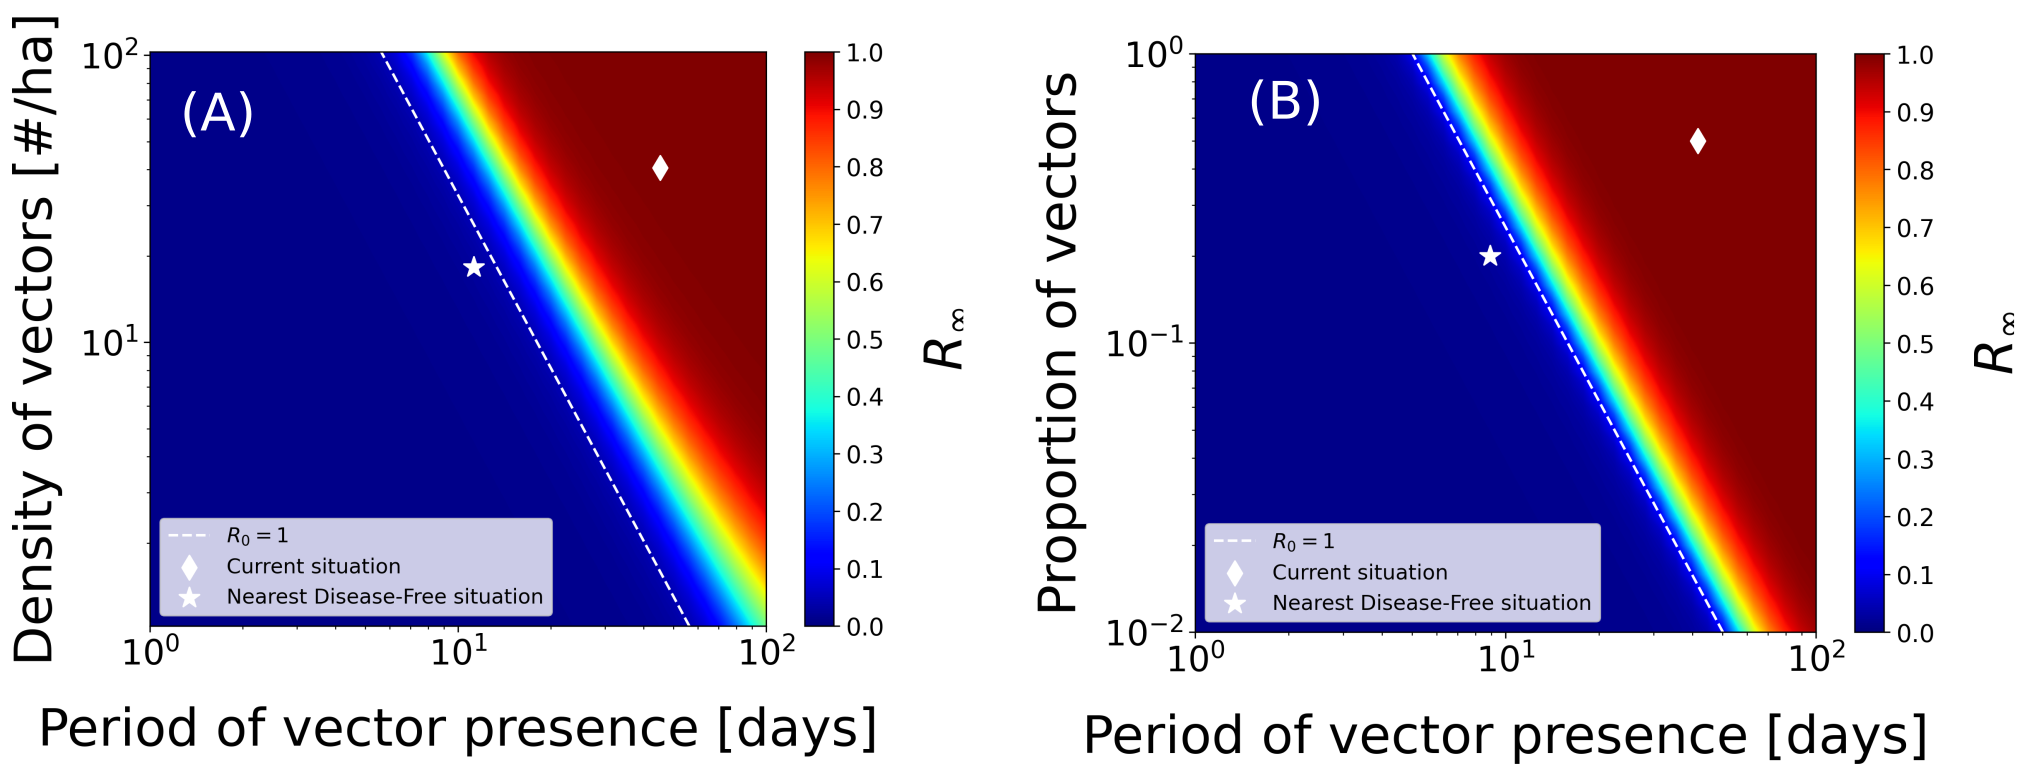
\includegraphics[width=\textwidth]{Figures/Control_strategy.png}
    \caption[Epidemic control through vector management for ALSD in Mallorca
        and
        OQDS in Apulia]{Epidemic control through vector management for ALSD in
        Mallorca (A) and OQDS in Apulia (B). The white shaded line denotes
        $R_0=1$, and the white diamond corresponds to the parameter values of
        the fitted model. The white star is the closest disease-free state to
        the current situation in this representation.}
    \label{fig:control_strategy}
\end{figure}

\section{Discussion}

In this work, we have developed a deterministic continuous-time
compartmental model for \textit{Xylella fastidiosa} vector-borne diseases in
Europe. The model attempts to characterize the main biotic processes that lead
to the development of epidemics, including the seasonal dynamics of the main
vector, \textit{P. spumarius}. We show how the model is sufficiently general to
represent with some accuracy the parameters that determine the ALSD in Mallorca
(Spain) and the OQDS in Apulia (Italy), both transmitted by \textit{P.
    spumarius}. To our best knowledge, this is the first mathematical model
describing Xf epidemics that considers the temporal pattern of vector abundance
observed in field data, faithfully representing the known biological
information about the pathosystem. It includes a dynamic approximation of the
non-stationary populations of \textit{P. spumarius}, mathematically represented
by a sporadic source term through which vectors are born every year, and an
exponential decay term. Due to the non-stationarity of the vector dynamics,
$R_0$ in the model cannot be computed with standard methods such as the Next
Generation Matrix \cite{Diekmann2010}. To circumvent this problem, we applied
an approximate method to compute it as previously proposed by
\cite{GimenezRomero2022_PRE}. We show that this approximate $R_0$ correctly
characterizes the epidemic, further validating the method proposed by
\cite{GimenezRomero2022_PRE}.

Nonlinear mathematical models of disease transmission enhance our
understanding of the different mechanisms operating in an epidemic, especially
compared with correlative or machine learning methods, often very useful in
practice but offering very little understanding. A key aspect to render these
models useful is the determination of the parameters from available data. If
this step can be properly performed, these models become very predictive and
especially helpful to design disease control strategies. However, an
appropriate calibration of the model relies on access to good-quality field
data, which is often the bottleneck for the application of this kind of models.
In the present study, the parameters have been obtained using a Bayesian
inference framework, which relies on probability distributions rather than
point-like measures. This way, mean or median values can be considered together
with their confidence intervals able to characterize the robustness of the
obtained parameters. In general, we obtained different values of the parameters
for the ALSD and OQDS outbreaks in Mallorca and Apulia, respectively. The
fitted values, however, are in good agreement with previous field-based
measures for each disease, while the differences observed between both
outbreaks may reflect differences between the Xf subspecies and crops involved
(deciduous vs. evergreen).

One of the conclusions of the study is that the available data for both
diseases is not enough to obtain robust estimates for all of the model
parameters. The lack of data about the vector population compartments yields
many possible values for the parameters that regulate transmission, $\alpha$
and $\beta$, provided that the progression of the host compartments correctly
fits the field data. In other words, very infectious vectors (high $\beta$)
that hardly ever get infected (low $\alpha$) can produce a similar outbreak
within the host population to that produced by very low infectious vectors (low
$\beta$) that get infected very often (high $\alpha$). The great difference in
these situations would be that, in the former, the infected vector population
would be very low, while in the latter, it would be quite high. This is a
manifestation of parameter unidentifiability from the fit
\cite{Chowel2017,Roosa2019}, which stresses the importance of transmission
and calls for detailed measurements of the vector population and not just of
the hosts. Furthermore, to compare transmission rates between different
diseases caused by Xf (e.g., $\beta$, $\alpha$), it is necessary to know the
vector-host population ratio of the pathosystem ($N_v/N_H$), since $\beta$ is
expressed as a number of hosts per vector per day. Although, in general,
populations of \textit{P. spumarius} in the canopy of olive trees are much
larger than those found in the almond trees of the Balearic Islands during the
months of July and August \cite{Lopez2021},
our work is based on data from studies in which information of the vector
populations is not provided. Without this information, therefore, conclusive
results regarding transmission cannot be obtained.

In any case, our model shows that the vector-to-plant transmission process,
mediated by $\beta$, is somehow different from that from the plant-to-vector
one, mediated by $\alpha$. In essence, $\beta$ must be smaller than $\alpha$ in
order to reproduce the observed outbreaks and have a sufficiently large vector
population getting infectious, being this fact independent of the particular
choice of $N_v(0)/N_H$. This heterogeneity can be caused by several factors:
differences in the efficiency of plant-to-vector transmission with respect to
vector-to-plant transmission; differences in contact rates, i.e., susceptible
vectors contact trees at a different rate than infected vectors; vector feeding
preferences, i.e., differences in the probability of contacting a susceptible
host compared to an infectious host, etc. Indeed, our mathematical model
assumes constant contact rates with no preferences over any host state, so that
under these assumptions, it indicates that the probability of effectively
transmitting the pathogen from plant to vector is greater than from vector to
plant. However, this interpretation is subject to this particular assumption,
so that to fully disentangle this question, experimental work in the form of
transmission assays should be performed. Furthermore, we found that the timing
and magnitude of the infectious host peak and the final number of dead hosts
are mostly controlled by the vector-to-plant transmission rate, $\beta$, the
plant-to-vector transmission rate, $\alpha$, and the vector removal rate,
$\mu$. Because these parameters are strongly related to the vector, the
analysis makes clear that enhancing the knowledge about the vector, as well as
obtaining precise data, is crucial to improve the modeling of Xf diseases and
pose important questions to be solved in specifically designed experiments.

The fact that the most influential parameters of the model are those
related to the vector can be used to design appropriate disease control
strategies. Because acting on transmission rates is rather cumbersome, we argue
that control strategies should focus on reducing the vector population in crop
fields. In our model, this depends on two parameters, $\mu$, the rate at which
vectors die (or move to herbaceous vegetation and other non-host trees or exit
the field), and $N_v(0)$, the number of newborn susceptible vectors every year
(assumed constant in this study). Our results show that a mixed strategy acting
on both parameters is optimal to lower disease prevalence and, eventually,
eradicate the disease. Interestingly, we also show that acting on the vector
removal $\mu$ is more effective than controlling the newborn vector population
$N_v(0)$. In fact, most control strategies carried out in practice for Xf
diseases focus on the latter factor, reducing $N_v(0)$ via egg or nymph control
\cite{Cornara2018, lopez2022mechanical, Lago2023}. However, our results
indicate that alternative strategies based on increasing the removal (or
dispersal) rate of vectors should be explored. Furthermore, the evolution of
the population compartments of the hosts and vectors provides relevant
information on the epidemiology of both diseases. In both cases, the newly
defined basic reproductive number that accounts for a decaying vector
population is very predictive of the moment in which new infections are not
produced anymore, coinciding approximately with the peak of infectious hosts.
Therefore, any intervention with control measures after this peak would have
marginal effects on future disease progression.

Our mathematical model is still rather simple, implementing only a few
relevant epidemic processes in contrast to the high complexity of the
pathogen-vector-host interactions occurring in plant epidemics. Indeed, the
model itself raises some questions about these interactions, for example,
whether contact rates are homogeneous. Another simplification of the
model is the fact that the spatial constraints and the intrinsic stochasticity
of the transmission processes are neglected. A straightforward extension of the
model would be to include a specific spatial setting and implement the explicit
motion of the vector within a stochastic framework, such as individual-based
models \cite{Grimm2005}. With this, the effectiveness of current and further
control strategies could be tested and improved controlling for the motion of
the vector. For instance, the control strategy based on the removal of
symptomatic trees together with their surrounding trees at a given distance
could be implemented in the model, evaluate the current effectiveness according
to the present protocols, and even provide improved parameters to be
implemented in the field. Of course, implementing a model in which the spatial
degrees of freedom are explicitly represented would require access to further
information about vector mobility and spatially resolved data to confront the
model, which is not currently available.

Mathematical models tested against experimental data increase our understanding
of the system under study. They also help to identify critical
parameters that require better prior information to adjust functions relating
to different variables and make the model predictions more accurate to suggest
and test control strategies \cite{cunniffe2015thirteen, jeger2018plant}. Our
mathematical model suggests a certain lack of knowledge of the transmission
processes and reveals that the currently available data is not enough to fit
complex models dealing with the explicit dynamics of the vector population.
